% The master copy of this demo dissertation is held on my filespace
% on the cl file serve (/homes/mr/teaching/demodissert/)

% Last updated by MR on 2 August 2001

\documentclass[12pt,twoside,notitlepage]{report}

\usepackage{a4}
\usepackage{verbatim}
\usepackage{units}
\usepackage{hyperref}
\usepackage{array}
\usepackage{listings}
\usepackage{parskip}
\usepackage{color}
\usepackage[usenames,dvipsnames]{xcolor}
\usepackage[noline,plain]{algorithm2e}
\usepackage{minibox}
\usepackage{amsfonts}
\usepackage{graphicx}
\usepackage{float}
\usepackage{soul}
\usepackage{hyperref}
\usepackage{paralist}
\usepackage{subfigure}

% \usepackage{dejavu}
% \usepackage{courier}
\usepackage[T1]{fontenc}

\input{epsf}                            % to allow postscript inclusions
% On thor and CUS read top of file:
%     /opt/TeX/lib/texmf/tex/dvips/epsf.sty
% On CL machines read:
%     /usr/lib/tex/macros/dvips/epsf.tex


\raggedbottom                           % try to avoid widows and orphans
\sloppy
\clubpenalty1000%
\widowpenalty1000%

\newcommand{\strAuthor}{David Brazdil}
\newcommand{\strCollege}{Trinity Hall}
\newcommand{\strTitle}{Taint-based Data Flow Analysis on Android}
\newcommand{\strExamination}{Computer Science Tripos, Part II}
\newcommand{\strYear}{June 2013}
\newcommand{\strSupervisor}{Dr A. Beresford}

\addtolength{\oddsidemargin}{6mm}       % adjust margins
\addtolength{\evensidemargin}{-8mm}

\renewcommand{\baselinestretch}{1.1}    % adjust line spacing to make
                                        % more readable
                                        

\newbox\subfigbox % Create a box to hold the subfigure.
\makeatletter
\newenvironment{subfloat}% % Create the new environment.
{\def\caption##1{\gdef\subcapsave{\relax##1}}%
\let\subcapsave=\@empty % Save the subcaption text.
\let\sf@oldlabel=\label
\def\label##1{\xdef\sublabsave{\noexpand\label{##1}}}%
\let\sublabsave\relax % Save the label key.
\setbox\subfigbox\hbox
\bgroup}% % Open the box...
{\egroup % ... close the box and call \subfigure.
\let\label=\sf@oldlabel
\subfigure[\subcapsave]{\box\subfigbox}}%
\makeatother

\newcommand{\centerbox}[1] {
	\begin{center}
	\begin{footnotesize}
	\begin{tabular}{l}
	#1
	\end{tabular}
	\end{footnotesize}
	\end{center}
}

\definecolor{lightOrange}{HTML}{FBD2AF}
\sethlcolor{lightOrange}
\definecolor{lightGreen}{HTML}{E3FFD5}
\sethlcolor{lightGreen}

\newcommand{\highlight}[1]{\colorbox{lightOrange}{\strut #1}}
\setlength{\fboxsep}{0pt}
\newcommand{\lsthl}[1] {\ttfamily\scriptsize\highlight{#1}}

\newcommand{\asm}[1] {\texttt{#1}}
\newcommand{\asmExtra}[1] {\texttt{\highlight{#1}}}

\newcommand{\tick}{$\checkmark$}
\newcommand{\cross}{$\times$}

\newcommand{\weblink}[1] {\footnote{\scriptsize\url{#1}}}

\setlength{\intextsep}{10pt}


\title{\strTitle}
\author{\strAuthor}

\begin{document}

\bibliographystyle{plain}

\lstset{
	language=Java,
	tabsize=2,
	basicstyle=\ttfamily\scriptsize,
	escapeinside=\`\`, %{\%*}{*)},
	captionpos=b,
	keywordstyle=\color[rgb]{0,0,1},
    commentstyle=\color[rgb]{0.133,0.545,0.133},
    stringstyle=\color[rgb]{0.627,0.126,0.941},	
}

%%%%%%%%%%%%%%%%%%%%%%%%%%%%%%%%%%%%%%%%%%%%%%%%%%%%%%%%%%%%%%%%%%%%%%%%
% Title


\pagestyle{empty}

\hfill{\LARGE \bf \strAuthor}

\vspace*{60mm}
\begin{center}
\Huge
{\bf \strTitle} \\
\vspace*{5mm}
\strExamination \\
\vspace*{5mm}
\strCollege \\
\vspace*{5mm}
\today  % today's date
\end{center}

\cleardoublepage

%%%%%%%%%%%%%%%%%%%%%%%%%%%%%%%%%%%%%%%%%%%%%%%%%%%%%%%%%%%%%%%%%%%%%%%%%%%%%%
% Proforma, table of contents and list of figures

\setcounter{page}{1}
\pagenumbering{roman}
\pagestyle{plain}

\chapter*{Proforma}

{\large
\begin{tabular}{ll}
Name:               & \bf \strAuthor \\
College:            & \bf \strCollege \\
Project Title:      & \bf \strTitle \\
Examination:        & \bf \strExamination, \strYear \\
Word Count:         & \bf \input{word_count}\footnotemark[1] \\
Project Originator: & \strSupervisor \\
Supervisor:         & \strSupervisor \\ 
\end{tabular}
}
\footnotetext[1]{This word count was computed
by {\tt detex -n diss.tex | tr -cd '0-9A-Za-z $\tt\backslash$n' | wc -w}
}
\stepcounter{footnote}

\section*{Original Aims of the Project}

To write a demonstration dissertation using \LaTeX\ to save
student's time when writing their own dissertations. The dissertation
should illustrate how to use the more common \LaTeX\ constructs. It
should include pictures and diagrams to show how these can be
incorporated into the dissertation.  It should contain the entire
\LaTeX\ source of the dissertation and the Makefile.  It should
explain how to construct an MSDOS disk of the dissertation in
Postscript format that can be used by the book shop for printing, and,
finally, it should have the prescribed layout and format of a diploma
dissertation.

\section*{Work Completed}

All that has been completed appears in this dissertation.

\section*{Special Difficulties}

None.
 
\newpage
\section*{Declaration}

I David Brazdil of Trinity Hall,\\
being a candidate for Part II of the Computer Science Tripos,
hereby declare that this dissertation and the work described in it
are my own work, unaided except as may be specified below, and
that the dissertation does not contain material that has already
been used to any substantial extent for a comparable purpose.

I give permission for my dissertation to be made available in the archive
area of the Laboratory's website.

\bigskip
\medskip
\leftline{Signed}

\bigskip
\leftline{Date}

\cleardoublepage

\tableofcontents

\newpage
\section*{Acknowledgments}

This document owes much to an earlier version written by Simon Moore
~\cite{moore95}.  His help, encouragement and advice was greatly 
appreciated.

%%%%%%%%%%%%%%%%%%%%%%%%%%%%%%%%%%%%%%%%%%%%%%%%%%%%%%%%%%%%%%%%%%%%%%%
% now for the chapters

\cleardoublepage        % just to make sure before the page numbering
                        % is changed

\setcounter{page}{1}
\pagenumbering{arabic}
\pagestyle{headings}

\chapter{Introduction}

Smartphones have grown to become very popular over the past few years as universal, always connected and increasingly affordable personal devices that users carry with them at all times. By integrating into many facets of our lives, we now trust smartphones with more and more sensitive data, making them attractive to criminals and marketing companies. According to a Bitdefender security specialist, nowadays one in three free applications on Android collects private data without user consent~\cite{web:HuffingtonOneInThree}. This dissertation presents one possible approach to building a system that monitors selected applications and warns the user when they attempt to leak private data. Dexter achieves this by modifying the executable code of an Android application to dynamically track data flow using a taint-based analysis.

\section{Problem Statement}

Applications for smartphones have access to a startling amount of personal information which is often highly beneficial to the user. They can access the contact list, calendar, call log, browser history or even the current location of the user, and combine these in novel ways that render everyday tasks simpler. But as studies have shown~\cite{web:Appthority, web:HuffingtonOneInThree}, applications can and \emph{do} misuse the permissions they were given in good faith, and leak collected data to remote servers where user has no control over them. These fall into three categories:
\begin{description}
\item \textbf{Data Stealing} \\
Due to Android's openness, it is not uncommon for programs to contain some form of malicious code. Usually these masquerade as legitimate applications but run a background trojan that sends premium text messages, logs keystrokes and sends data useful for spamming or identity theft to its authors. Malware is present mainly on alternative markets and in illegal pirated software~\cite{Zhou:2012:DRS:2133601.2133640}, but from time to time appears even on the official store~\cite{web:LookoutPlayRemoval}.

\item \textbf{Mismatch of Expectations} \\
Behaviour that is not deliberately malicious but might pose security risks defines a group of applications referred to as \emph{grayware}. These are typically advertising libraries which collect private data in order to uniquely identify the person and to show tailored ads, all without an adequate warning.

\item \textbf{Accidental Permissions} \\
Sometimes applications request access to more resources than they need by mistake. A cautious user might want to do preventive monitoring. 
\end{description}

Current state of the art in smartphone data protection lags behind the practices described above. Android developers can freely publish applications on the official store, but they might be removed if red-flagged by the automatic Bouncer~\cite{web:Bouncer} or by third parties~\cite{web:LookoutPlayRemoval}. During installation the user is merely shown a list of requested permissions, without any justification of their necessity. The situation is slightly better on iOS, where each application must pass a manual approval process before being published. Users also grant per-resource access when requested for the first time, providing some context in which data are needed.

Nevertheless, both of these policies fail to protect against applications that have a legitimate initial reason to read private data but secretly leak it too, since once granted access, use of a resource is unrestricted.

\section{Project Overview}

Taint-based dynamic data flow analysis is a technique to examine the runtime behaviour of applications. It is capable of monitoring access to resources and identifying data paths between them. It was previously successfully implemented on other platforms~\cite{Zhu:2011:TPS:1945023.1945039}, and recently ported to Android in the TaintDroid project~\cite{web:TaintDroid, Enck:2010:TIT:1924943.1924971}, a joint study by Intel Labs, Penn State, and Duke University. However, their solution involves changes to the operating system and its virtual machine, limiting its usage to experts in possession of one of few supported devices. The goal of this project was to implement taint analysis by modifying the application rather than the operating system, to make it easier to employ.

\subsection{Data Flow Analysis}

\begin{figure}
	\centerline{	
		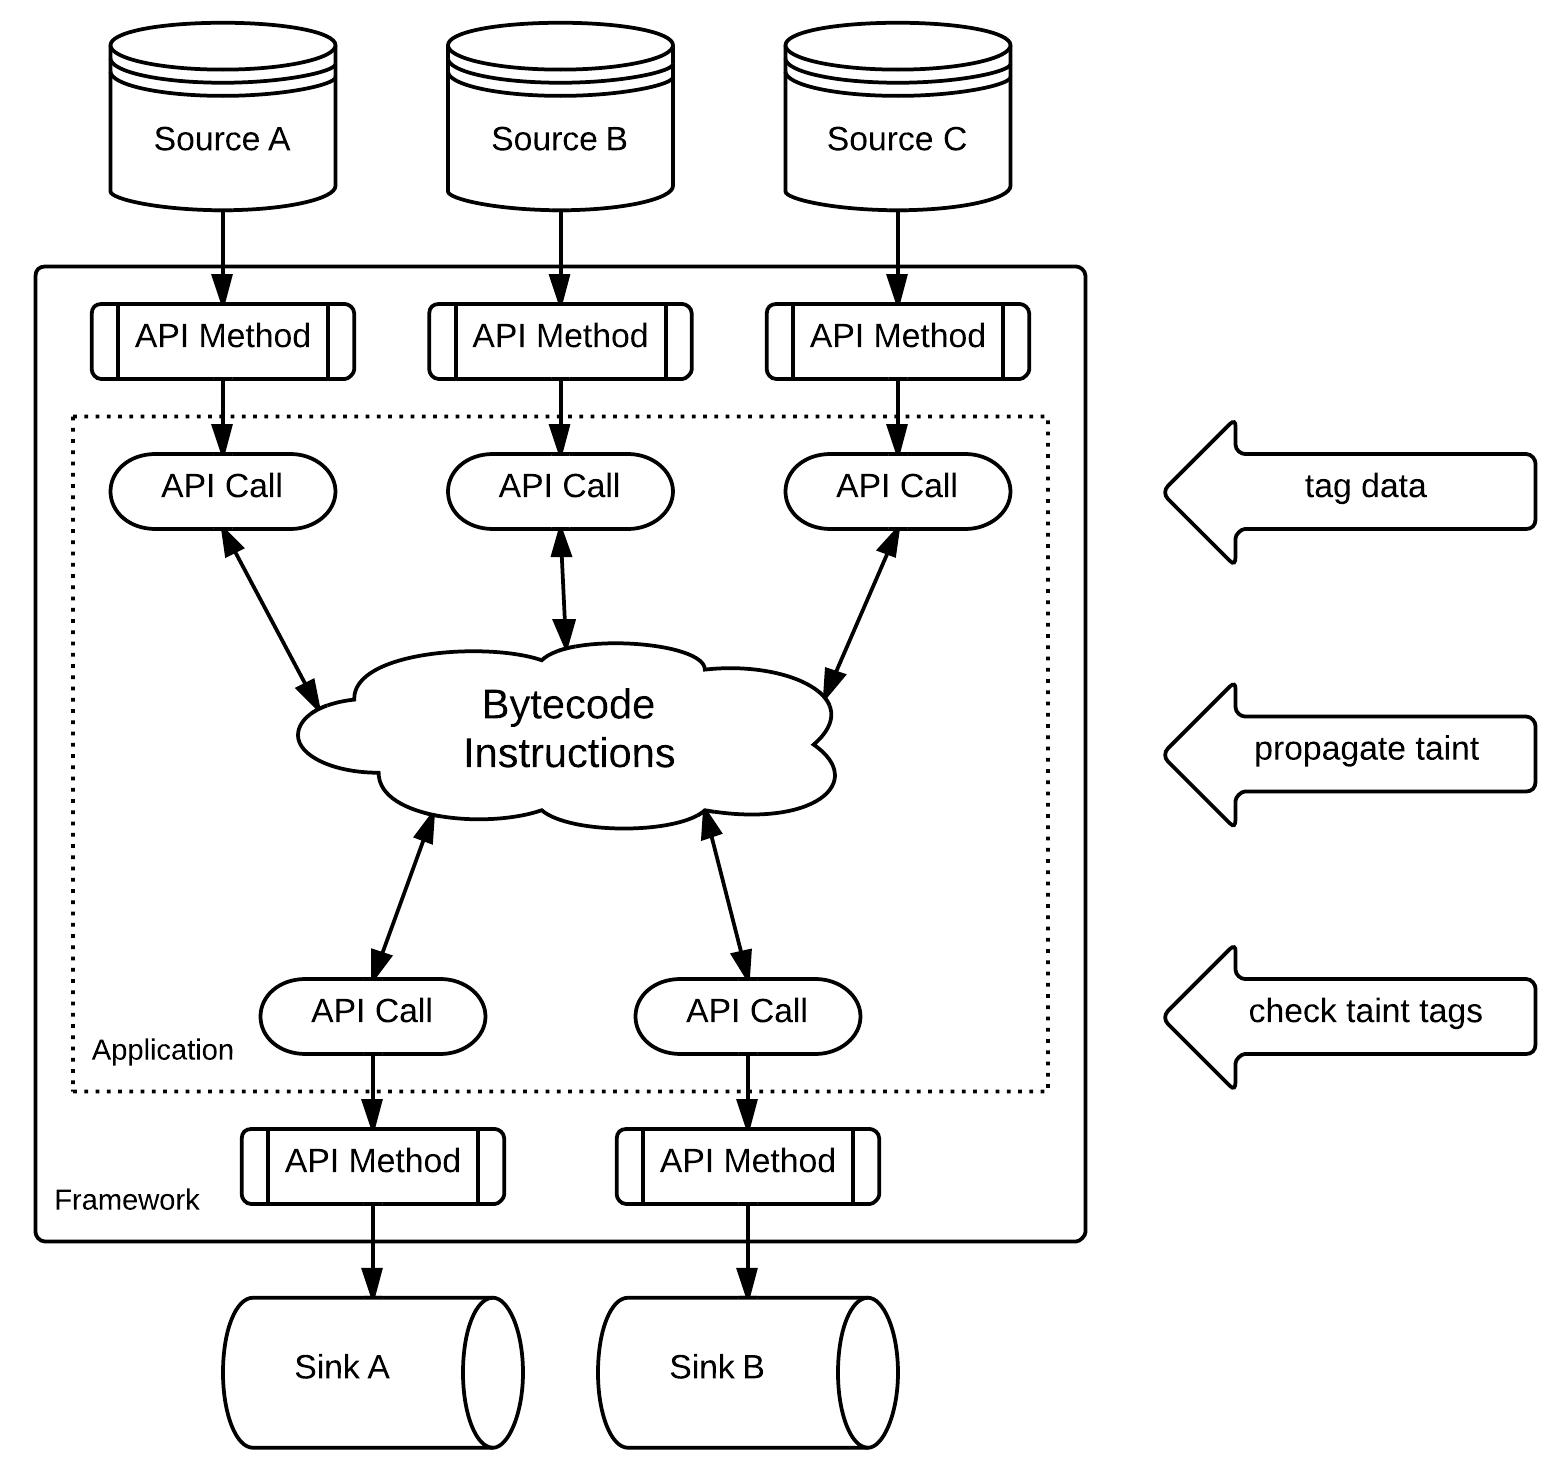
\includegraphics[width=0.8\textwidth]{figs/fig_intro_tainting.png}
	}
	\caption{Overview of the taint analysis.}
	\label{fig:Introduction_TaintingOverview}
\end{figure}

Dynamic taint analysis relies on the ability to assign attributes, called \emph{taint tags}, to data in memory. In our context, these represent whether the memory location stores private information. Execution of the program is altered so that tags are assigned to tracked data at the points of their origin, known as \emph{sources}, and output points, \emph{sinks}, are monitored to make sure no tainted data leave the system. For example, sources and sinks on Android include the contacts database and network sockets respectively. In between, tags are propagated as data are moved and combined. 

The approach adopted by TaintDroid monitors sources and sinks at the kernel level and requires modifications to the VM and the file-system to propagate taint. This allows it to track data flow throughout all of interpreted code, even between applications. Limited by the boundaries of the VM, Dexter performs the analysis only within a single application by instrumenting its executable file, which we call the \emph{internal code}. Resources are monitored at the points of respective API calls, which form the border between tracked and untracked code. Stages of the analysis are summarized in Figure~\ref{fig:Introduction_TaintingOverview}. 

Of course tainting brings complications as well. Most notably, it often struggles to avoid \emph{taint explosion}, an uncontrollable spread of taint due to conservative propagation logic resulting in false positives. Nearly all such systems also entirely ignore \emph{implicit data flows}, i.e.\ propagation of data through control flow such as the implicit flow of data between \texttt{y} and \texttt{x} in "\verb$while (x--) y++;$". Attempts have been made to identify such constructs through static analysis~\cite{Nair:2008:VMB:1346355.1346524}, but these are prone to taint explosion. Further details about tainting can be found in~\cite{Schwartz:2010:YEW:1849417.1849981, Ermolinskiy:EECS-2010-92}.

\subsection{Usage of Dexter}

% \begin{figure}
% 	\centerline{	
% 		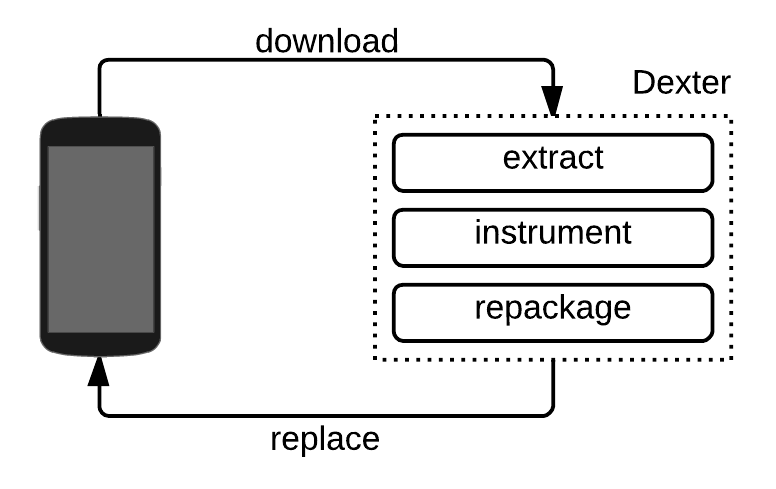
\includegraphics[width=0.5\textwidth]{figs/fig_intro_overview.png}
% 	}
% 	\caption{Principle of application replacement with its instrumented version.}
% 	\label{fig:Introduction_AppReplacement}
% \end{figure}

From the user's perspective, the process of application protection enhancement is simple. A smartphone is connected to a PC running Dexter, and the user is presented with a list of applications installed on the device. The selected app is downloaded into the computer, instrumented, repackaged and uploaded back to the device where it replaces its original counterpart. This application then runs the taint analysis in the background and warns the user when tainted data reaches a monitored sink. In the future, Dexter could be shipped as an app and run on the device itself.

Even though the aim of Dexter is to make TaintDroid functionality available on every Android device, it is still a tool that only security experts and cautious power users would use. Its biggest potential however lies in the enterprise sector, protecting corporate data on personal phones of the employees, much like increasingly popular \emph{app wrapping}~\cite{web:AppWrapping}. With some modifications it could also replace TaintDroid as the flow tracking component inside CleanOS~\cite{Tang:2012:CLM:2387880.2387888}, another security-enhancing project that prevents data theft.

\section{Related Work}

The community around Android has built an entire ecosystem of tools that help security experts analyze and reverse-engineer applications, and grouped them into the HoneyNet project\weblink{http://www.honeynet.org/}. The core of these tools is usually formed by the Smali\weblink{https://code.google.com/p/smali/} (dis)assembler and the Androguard\weblink{https://code.google.com/p/androguard/} static analysis framework. Of particular significance to professionals are APKInspector\weblink{https://github.com/honeynet/apkinspector}, which provides useful behavioural information through static taint analysis~\cite{2012kim_scandal}, and DroidBox\weblink{https://code.google.com/p/droidbox/}, a sandboxed emulator environment with resource monitoring. 

In terms of techniques, a lot of attention has been paid to automated malware detection, in order to instantly prevent its distribution through both the official and alternative market stores. Projects like RiskRanker~\cite{Grace:2012:RSA:2307636.2307663} and DroidRanger~\cite{Yajin:12NDSS} look for behavioural patterns common to known spyware and malware, while for example DroidMoss~\cite{Zhou:2012:DRS:2133601.2133640} focuses on identifying repackaged applications that could have been trojanized. 

Another large set of projects, including TaintDroid, puts effort into enhancing the runtime privacy policies of the platform. For instance, MockDroid~\cite{Beresford:2011:MTP:2184489.2184500} allows fine-grained permission removal through resource mocking, and Aurasium ~\cite{Xu:2012:APP:2362793.2362820} can intercept and prevent interactions of applications with the OS by repackaging them in order to insert its monitor between the kernel and the VM. In the enterprise sector, virtualization~\cite{web:Virtualization} and app wrapping~\cite{web:AppWrapping} are gaining popularity as ways of creating a separate corporate workspace on personal devices.

\cleardoublepage
\chapter{Preparation}

\section{Dalvik Virtual Machine}

Dalvik is an open-source virtual machine and an essential component of the Android operating system. It was developed specifically for use on mobile devices and its design was optimized for running on battery-powered systems with low-performance processor and limited memory. 

Built around the Apache Harmony project, Dalvik runs programs that make use of a subset of the Java runtime framework. Applications for Dalvik are therefore typically written in Java, compiled to a set of Java Virtual Machine (JVM) bytecode \emph{.class} files, and then converted to a single Dalvik-compatible \emph{.dex} file~\cite{web:DalvikDex} using tools in the Android SDK. With release 2.2, Dalvik introduced Just-In-Time compilation which significantly increased its performance and efficiency~\cite{web:DalvikJit}.

\subsection{Application Package Files}

Applications are distributed in Android Package (APK) files. These are ZIP files signed by the publisher, which contain:
\begin{inparaenum}[(i)]
\item \emph{classes.dex} executable file,
\item application resources (images, UI layouts, ...),
\item native code binaries, and
\item a manifest.
\end{inparaenum}

The manifest contains essential information about the application to the operating system. Among other things, this includes its unique package name, list of permissions requested by the application, and a list of all its entry points.

APKs are stored on the device when applications are downloaded from the market or installed manually, and can be retrieved from the device only with root access. Instrumented files can be installed on any device. 

\subsection{Bytecode}

Dalvik bytecode is very similar to that of the JVM in the sense that they both have a large set of rather high-level instructions~\cite{web:DalvikBytecode, web:JavaBytecode}, making it more readable and more easily modified than traditional instruction sets, unless obfuscation tools like ProGuard\weblink{https://developer.android.com/tools/help/proguard.html} are used. This makes analysis and reverse-engineering of applications significantly easier, and is also the reason why we will freely interchange examples in assembly and Java.

\subsubsection{Registers}

Unlike the stack-based JVM, Dalvik uses a register-based programming model with 32-bit register width and variable-length instructions~\cite{web:DalvikInsnFormat}. 64-bit values are stored in two adjacent registers.

Each method can use up to 65,536 virtual registers mapped either to hardware registers or stack memory depending on the underlying architecture. 
% On a typical Android device, the first 16 virtual registers would map to the 16 registers available in the ARM instruction set, and rest would be stored in memory. 
Instructions can address either the first 16, 256, or all 65k virtual registers based on their length. If an instruction needs to address a register out of the available range, the register contents are expected to get moved to a lower register first.

Dalvik also has a very powerful preload class verifier~\cite{web:DalvikVerifier, web:DalvikDexopt}. It infers types of values in registers at every point in computation, and uses these to identify illegal access to resources, pointer arithmetic and other invalid operations. A~class containing such instructions is rejected and the application terminated.

\subsubsection{Syntax of Assembly}

The assembly language syntax used in this dissertation is based on the official Dalvik one~\cite{web:DalvikBytecode}. It follows the \emph{dest-then-source} ordering of arguments, and instructions can contain immediate values, e.g.\ the instruction
		\centerbox{
			\asm{add-int/lit16 v2, v8, \#1234}
		}
adds 1234 to the value stored in register 8, and stores the result into register 2. 

Since actual numerical register identifiers are irrelevant to the propagation logic we will treat them as variables. For example the following piece of code retrieves an element of an array pointed to by \verb$vArray$, and multiplies it by three:
	\begin{figure}[H]
		\centerbox{
			\asm{aget-int vElement, vArray, vIndex} \\
			\asm{mul-int/lit16 vResult, vElement, \#3}
		}
	\end{figure}

For clarity, the first letters of register names will represent their origin. Names of registers used in the original code will start with \verb$r$, registers added for tainting with \verb$t$, and auxiliary registers with \verb$p$.

Register pairs forming a wide argument will be separated by a bar:
	\begin{figure}[H]
		\centerbox{
			\asm{move-wide rTo1 | rTo2, rFrom1 | rFrom2}
		}
	\end{figure}

\subsubsection{Instruction Variants}

To achieve higher code density, some Dalvik instructions come in several variants~\cite{web:DalvikBytecode}. They are semantically equivalent but they differ in size. A good example of this is the \verb$const$ instruction. Its variant \verb$const/16$ stores a 16-bit constant into a register addressed by an 8-bit number, and therefore the whole instruction fits into 4 bytes. On the other hand, \verb$const/4$ fits into 2 bytes, but can only address registers in the 4-bit range and carry a 4-bit constant.

All variants of semantically equivalent instructions are parsed as the same instruction type in Dexter, and thus will be referred to by the same name. During the reassembly phase, Dexter automatically outputs the most optimized variant of the instruction.

\section{Data Flow Analysis}
\label{section:DataFlowAnalysis}

\subsection{Taint Tags}

Different tainting systems choose different ways of representing tags. This fundamental choice has a large effect on the overall design of the system, its capabilities and limits, as well as performance and memory overhead. The authors of TaintDroid decided to store taints as 32-bit integers where each bit represents one source of sensitive data. This is a very efficient and compact format, sufficient for the purposes of TaintDroid, but quickly reaches its limits as the functionality is extended. One of the challenges faced by the CleanOS project~\cite{Tang:2012:CLM:2387880.2387888}, which builds on TaintDroid, was the necessity to potentially track millions of taint sources. Their solution alters TaintDroid to store taint as a 32-bit pointer into an SQL database, which increases the number of trackable sources, but significantly impedes performance. 

Dexter adopts the same tag representation as TaintDroid, with one modification. As will be demonstrated later, the type of sink formed by some API calls is given by the way their containing object was created. Tags therefore have flags reserved to carry this information. The flags in taint as used in Dexter are summarized in Table~\ref{table:TaintTagStorage_BitMeaning}.

\begin{table}
	\begin{center}
	\begin{tabular}{|c|l|l|}
		\firsthline
		\textbf{Bit} & \textbf{Constant name}        & \textbf{Description} \\
		\hline
		0            & \verb$TAINT_SOURCE_CONTACTS$  & contact information \\
		1            & \verb$TAINT_SOURCE_SMS$       & text message data \\
		2            & \verb$TAINT_SOURCE_CALL_LOG$  & call history information \\
		3            & \verb$TAINT_SOURCE_LOCATION$  & location information \\
		4            & \verb$TAINT_SOURCE_BROWSER$   & browser data, e.g.\ bookmarks \\
		5            & \verb$TAINT_SOURCE_DEVICE_ID$ & device ID, e.g.\ IMEI, phone number \\
		\hline
		29           & \verb$TAINT_SINK_FILE$        & file-system sink \\
		30           & \verb$TAINT_SINK_SOCKET$      & network sink \\
		31           & \verb$TAINT_SINK_OUT$         & standard console output sink \\
		\lasthline
	\end{tabular}
	\end{center}
	\caption{Meanings of bit flags of taint tags}
	\label{table:TaintTagStorage_BitMeaning}
\end{table}

\subsection{Tag Storage}

To store and propagate taint tags, Dexter must build an attribute system inside the application, so that every piece of data accessible by internal code can carry one. The way these are stored differs for objects and primitives. The distinction is that when a primitive is copied, operations on one of the copies do not effect the other, which means that there has to be a tag stored for every copy, while when a reference to an object is copied, operations on one of the copies are visible by dereferencing any of them, and so there should only be one tag per object, not for every copy of its reference. 

\subsubsection{Objects}
\label{section:TaintTagStorage_Objects}

Dexter stores tags with objects by creating a globally accessible hash map from object references to integers. The only supported operations are:
\begin{description} 
\item \verb$int get(Object obj)$ \\
Returns the taint tag of given object, or zero when \verb$obj == null$.
\item \verb$void set(int taint, Object obj)$ \\
Adds taint to \verb$obj$ by OR-ing its existing entry with the first parameter. Does nothing when \verb$obj == null$.
\end{description}

In the following sections, the \verb$taint-get$ and \verb$taint-set$ macros (see section~\ref{section:Code_Macros}) will be used as a shorthand for calling these methods. 
	\begin{figure}[H]
		\centerbox{
			\asm{taint-get vResult, vObject} \\
			\asm{taint-set vTaint, vObject}
		}
	\end{figure}

\subsubsection{Primitives}

\label{section:TaintStorage_Primitives}

A taint tag needs to be created whenever a primitive is stored, i.e.\ for method code registers, primitive class fields and primitive arrays. Taint tags of parameters are also temporarily stored during method calls~(section~\ref{section:TaintPropagation_MethodCalls_Internal}).

\begin{itemize}

\item \textbf{method code registers} \\
For every register that appears in the original bytecode, Dexter creates a new one for storing taint. Doubling the number of registers is why Dexter needs to reallocate registers after instrumentation, otherwise some instructions might not be able to address these new registers.

\item \textbf{internal class fields} \\
Classes defined internally can be fully modified by Dexter. For every field of primitive type, a new field of type \verb$int$ is created, with a name that does not clash with any of the existing fields.

\item \textbf{external class fields} \\
Extra fields cannot be inserted into external classes and therefore a different approach must be adopted. 
\begin{itemize}
\item \textit{static fields} \\
A new class is created to contain one field of type \verb$int$ for every external static field that is accessed by the application. Taint tags are stored in these associated fields.

\item \textit{instance fields} \\
We will see that the propagation logic cannot assign tags to external instance fields for safety and uses the overall tag of the containing object instead. Storage space for these fields is therefore not needed.

\end{itemize}

\item \textbf{arrays} \\
Primitive array elements are considered equivalent to external instance fields under Dexter's propagation logic, and thus taint is assigned to the array object.

\end{itemize}

\subsection{Principles of Taint Propagation}

Once taint storage is created, Dexter can insert extra instructions that will propagate taint as data are used. Dalvik supports 217 opcodes, but these can be split into groups sharing the same propagation logic. The general rule of thumb is that for every instruction, taint of all its inputs should be acquired from their respective storage spaces, combined and assigned to the outputs. Therefore, only a handful of examples will be presented here to illustrate the principle and to explain some of the subtleties.

The following sections will contain examples of instrumentation, first in Dalvik assembly and later in Java for readability. Instrumentation of individual instructions will always be highlighted in green, longer listings of inserted code will be labelled.

\subsubsection{Constants}

Constants are not tainted, and so zero is stored in the appropriate taint register.

	\begin{figure}[H]
		\centerbox{
			\asm{const rTo, \#num} \\
			\asmExtra{const tTo, \#0}
		}
	\end{figure}

\subsubsection{Instructions Combining Taint}

Arithmetic instructions are the simplest example of taint tag combination. Tags of operands are OR-ed and this combined tag assigned to the result.

	\begin{figure}[H]
		\centerbox{
			\asm{add-int~rResult, rOpA, rOpB} \\
			\asmExtra{or-int~~tResult, tOpA, tOpB}
		}
	\end{figure}

\subsubsection{Instructions Operating on Wide Registers}

Taint of 64-bit primitives is stored only in the taint register of the higher of the two original registers holding the value. This is safe because accessing only one of them as a single-width register is an illegal operation. Classes containing such instruction will be rejected by Dalvik's preload class verifier.

	\begin{figure}[H]
		\centerbox{
			\asm{add-long rResult1 | rResult2, rOpA1 | rOpA2, rOpB1 | rOpB2} \\
			\asmExtra{or-int~~~tResult1, tOpA1, tOpB1}
		}
	\end{figure}

\subsubsection{Instructions Throwing Exceptions}

Some of Dalvik instructions can throw exceptions depending on the values of arguments. This is a form of implicit data flow which could potentially leak data. For example, integer division will throw \verb$ArithmeticException$ iff the divisor is zero, making this information deducible from the fact that the exception was thrown. Such instructions are wrapped in a try block, and the exception caught, tainted and thrown again.

	\begin{figure}[H]
		\centerbox{
			\asmExtra{TRY (ArithmeticException $\Rightarrow$ CATCH\_ABC) \{} \\
			\asm{~~div-int rResult, rOpA, rOpB} \\
			\asmExtra{~~or-int tResult, tOpA, tOpB~~~~~~~~~~~~} \\
			\asmExtra{~~goto LABEL\_XYZ~~~~~~~~~~~~~~~~~~~~~~~~} \\
			\asmExtra{\}~~~~~~~~~~~~~~~~~~~~~~~~~~~~~~~~~~~~~~~} \\
			\asmExtra{CATCH\_ABC:~~~~~~~~~~~~~~~~~~~~~~~~~~~~~~} \\
			\asmExtra{move-exception pException~~~~~~~~~~~~~~~} \\
			\asmExtra{taint-set tOpB, pException~~~~~~~~~~~~~~} \\
			\asmExtra{throw pException~~~~~~~~~~~~~~~~~~~~~~~~} \\	
			\asmExtra{LABEL\_XYZ:~~~~~~~~~~~~~~~~~~~~~~~~~~~~~~}
		}
		\caption{Example instrumentation of the division instruction}
		\label{figure:TaintPropagation_ThrowingInstructions}
	\end{figure}

\subsection{Method Call Destination Decidability}
\label{section:TaintPropagation_DestDecision}

The five types of method invocation supported by Dalvik are listed in Table~\ref{table:TaintPropagation_MethodCallTypes}. Instrumentation of each varies in detail
, but for tainting it is more important to know whether the target method lies inside the DEX file, in which case taint should be propagated into it, or whether it jumps into external, untrackable code and the instrumentation should therefore assign taint conservatively, assuming the worst, i.e.\ the method will spread taint everywhere it can.

\begin{table}[h]
	\begin{center}
	\begin{tabular}{|l|c|l|}
		\firsthline
		\textbf{Opcode}         & \footnotesize{\textbf{vtable}} & \textbf{Usage} \\
		\hline
		\verb$invoke-direct$    & \cross          & method a constructor or declared \verb$private$ \\
		\verb$invoke-static$    & \cross          & method declared \verb$static$ \\
		\hline
		\verb$invoke-virtual$   & \tick           & standard virtual method call \\
		\verb$invoke-interface$ & \tick           & method declared in an interface \\
		\verb$invoke-super$     & \tick           & call to closest parent implementing the method \\
		\lasthline
	\end{tabular}
	\end{center}
	\caption{Method call types supported by Dalvik}
	\label{table:TaintPropagation_MethodCallTypes}
\end{table}

\begin{figure}
	\centerline{	
		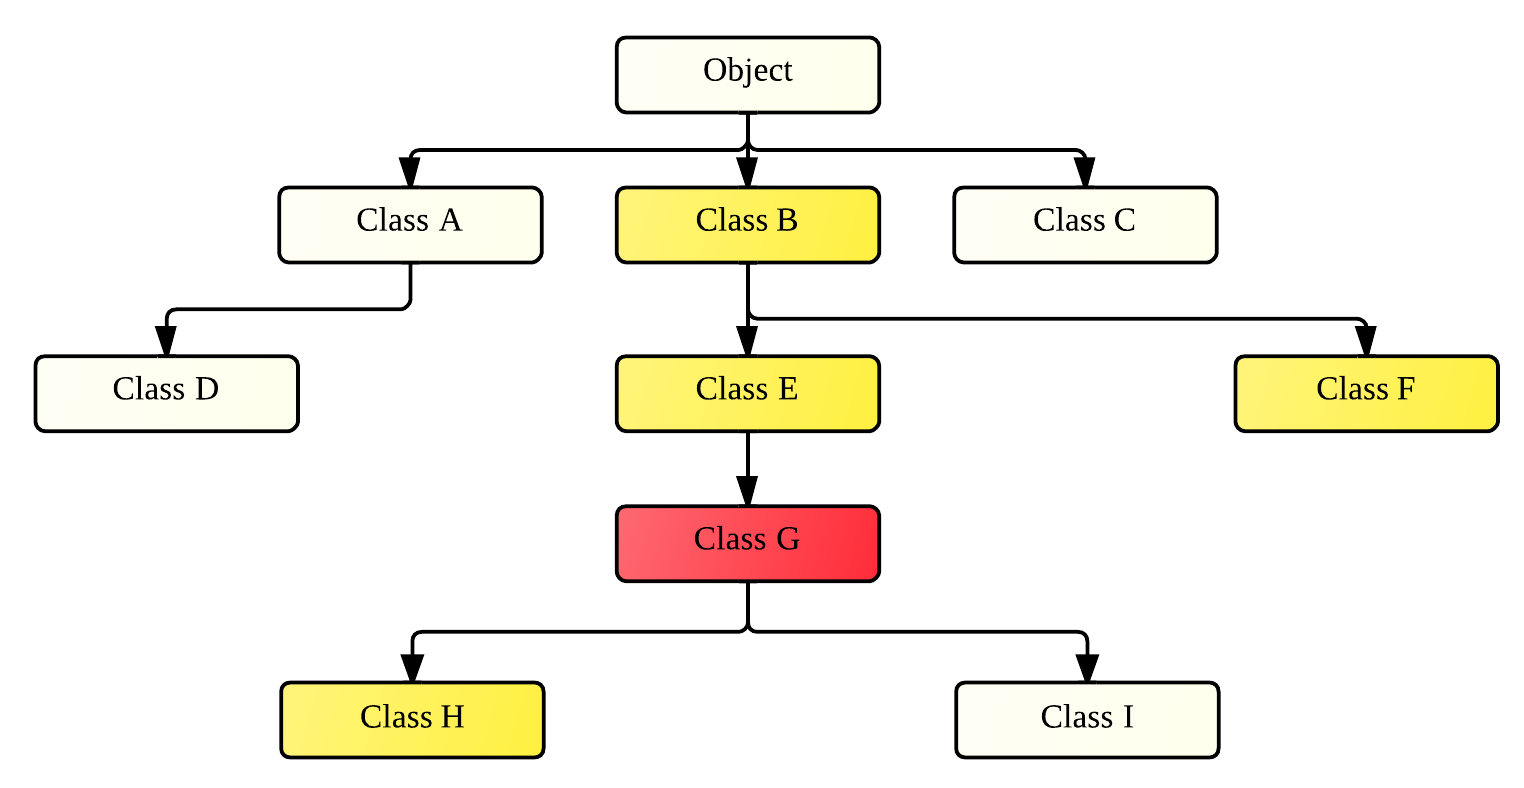
\includegraphics[width=0.7\textwidth]{figs/fig_virtual_call_tree.png}
	}
	\caption{Example class hierarchy for a method call.}
	\label{fig:TaintPropagation_DestDecision_ClassHierarchy}
\end{figure}

Determining the destination of a method call is trivial for \verb$invoke-direct$. The method signature always contains the name of the class implementing the method. Thus, it will perform an internal jump iff the referenced class is internal.

Only slightly more complicated is the case of \verb$invoke-static$ calls. The reason being that the method might not be implemented directly in the referenced class, but inherited from a parent, which renders the referenced class internality check insufficient. Dexter must check whether the class indeed implements the method and recursively explore parents if not.

All the other calls rely on dynamic dispatch, and since they are similar in principle, only the \verb$invoke-virtual$ case is discussed here. Imagine class hierarchy like the one in Figure~\ref{fig:TaintPropagation_DestDecision_ClassHierarchy}. The instruction calls a method defined in class $B$ and overridden in the yellow classes, on objects of type $G$ or its children. By the nature of virtual calls, the only implementations of the method that can be called are either in the closest parent that provides one or in the expected class and its children, that is $E$ and $H$ in the example. If these classes are all internal or all external, the destination type is decidable statically. 

\begin{figure}
	\centering
	\begin{tabular}{c}
	\begin{lstlisting}
// original code: obj.methodName(arg1, arg2, ..., argN)
Class c = obj.getClass();
Class[] argTypes = new Class[] { arg1.class, ..., argN.class };

Method m = null;
while (m == null) {
	try {
 		m = c.getDeclaredMethod("methodName", argTypes);
 	} catch (NoSuchMethodException e) {
 		c = c.getSuperclass();
 	}
}

Annotation a = m.getAnnotation(InternalMethodAnnotation.class);
if (a == null) {
	// external call
	obj.methodName(arg1, ..., argN);
} else {
	// internal call
	obj.methodName(arg1, ..., argN);
}
	\end{lstlisting}
	\end{tabular}
	\begin{lstlisting}[caption={Destination-deciding instrumentation for non-public methods},
	                   label={listing:TaintPropagation_MethodCall_DestDecidability_NonPublic}]
	\end{lstlisting}
\end{figure}

Code could be further analyzed to narrow down the number of callable implementations, e.g.\ by reachability analysis, but it will always be possible to produce code with a statically undecidable call. Then it is necessary to instrument the code so that the decision can be made at runtime. Dexter adds a special annotation to every method defined inside the application, which makes internal and external implementations dynamically distinguishable by reflection. A slight subtlety comes from the fact that the reflexive API handles public and non-public instance methods differently. Code for non-public methods is shown in Listing~\ref{listing:TaintPropagation_MethodCall_DestDecidability_NonPublic}. Instrumentation of public methods uses \verb$Class.getMethod$ to get \verb$m$ and does not need iteration through parents. It is nonetheless obvious that these are both very expensive operations. 

A native method is always marked as an external call.

\subsection{External Method Calls}
\label{section:TaintPropagation_MethodCalls_External}

External method calls are the border between trackable and untrackable code, and as such, their instrumentation will have to propagate taint conservatively, accounting for every possible action that the untrackable code could do. The approach adopted by Dexter is simple: the taint of all parameters is combined and assigned to the result and all \emph{mutable} parameters. The assumptions made here are that the method can access only data passed to it, and that it can return them or move them into any mutable parameter. If this proves to cause problematic over-tainting in some cases, Dexter offers a way of defining custom policies.

Unfortunately, these assumptions are not safe, as we can see in Listing~\ref{listing:ExternalMethodCalls_LogicHole}. The logic hole depends on the external environment providing a class that stores data inside invisible fields and then accesses and \emph{leaks} these data. From the Android documentation, it seems that sinks currently identified by Dexter do not have this property. However, it could be abused by serializing the object and leaking the untainted byte array. A solution to this problem would be to unify taints of interacting objects, so that tainting \verb$objB$ would automatically taint \verb$objA$ because they interacted on the previous line. But this could easily result in taint explosion.

\begin{figure}[H]
	\centering
	\begin{tabular}{c}
	\begin{lstlisting}
ClassA objA = new ClassA();     // external class
ClassB objB = new ClassB();     // internal class
objA.setX(objB);                // store B inside A
objB.setY(getSensitiveData());  // taint B
objA.useX();                    // use B inside
	\end{lstlisting}
	\end{tabular}
	\begin{lstlisting}[caption={Example of a propagation logic hole},
	                   label={listing:ExternalMethodCalls_LogicHole}]
	\end{lstlisting}
\end{figure}

\begin{figure}
	\centering
	\begin{tabular}{c}
	\begin{lstlisting}
// method definition
public int externalMethod (Object rArg1, int rArg2, String rArg3);

// method call
`\lsthl{int taintCombined = TaintMap.get(obj);~~~}`
`\lsthl{taintCombined |= TaintMap.get(rArg1);~~~~}`
`\lsthl{taintCombined |= tArg2;~~~~~~~~~~~~~~~~~~}`
`\lsthl{taintCombined |= TaintMap.get(rArg3);~~~~}`
`\lsthl{~~~~~~~~~~~~~~~~~~~~~~~~~~~~~~~~~~~~~~~~~}`
`\lsthl{try \{~~~~~~~~~~~~~~~~~~~~~~~~~~~~~~~~~~~~}`
`\lsthl{~~TaintMap.set(taintCombined, rArg1);~~~~}`
	rResult = obj.externalMethod(rArg1, rArg2, rArg3);
`\lsthl{~~tResult = taintCombined;~~~~~~~~~~~~~~~}`
`\lsthl{\} catch-all (rException) \{~~~~~~~~~~~~~~~}`
`\lsthl{	TaintMap.set(taintCombined, rException);}`
`\lsthl{	throw rException;~~~~~~~~~~~~~~~~~~~~~~~}`
`\lsthl{\}~~~~~~~~~~~~~~~~~~~~~~~~~~~~~~~~~~~~~~~~}`
	\end{lstlisting}
	\end{tabular}
	\begin{lstlisting}[caption={Instrumentation of external method calls. The second and third arguments do not inherit combined taint because they are immutable.},
	                   label={listing:TaintPropagation_ExternalMethodCall}]
	\end{lstlisting}
\end{figure}

\subsection{Internal Method Calls}
\label{section:TaintPropagation_MethodCalls_Internal}

\begin{figure}
	\centering
	\begin{tabular}{c}
	\begin{lstlisting}
// method definition
public int internalMethod (Object rArg1, float rArg2, short rArg3) {
	bool internalOrigin;

	// origin-deciding instrumentation
	StackTraceElement[] stack = (new Exception()).getStackTrace();
	if (stack.length > 1) {
		Class caller = Class.forName(stack[1].getClassName());
		callerAnnotation = caller.getAnnotation(InternalClassAnnotation.class);
		internalOrigin = (callerAnnotation != null);
	} else
		internalOrigin = false;

	// initialization of taint registers
	if (internalOrigin) {
		tArg2 = InternalMethodCall.ARG[0];
		tArg3 = InternalMethodCall.ARG[1];
		InternalMethodCall.S_ARG.release();
	} else {
		int thisTaint = TaintMap.get(this);
		TaintMap.set(thisTaint, rArg1);
		tArg2 = thisTaint;
		tArg3 = thisTaint;
	}

	// original method body
	... 
	`\lsthl{if (internalOrigin) \{~~~~~~~~~~~~~~~}`
	`\lsthl{	InternalMethodCall.S\_RES.acquire();}`
	`\lsthl{	InternalMethodCall.RES = tResult;~~}`
	`\lsthl{\}~~~~~~~~~~~~~~~~~~~~~~~~~~~~~~~~~~~}`
	return rResult;
}

// method call
`\lsthl{InternalMethodCall.S\_ARG.acquire();}`
`\lsthl{InternalMethodCall.ARG{[}0] = tArg2;~}`
`\lsthl{InternalMethodCall.ARG{[}1] = tArg3;~}`
rResult = obj.internalMethod(rArg1, rArg2, rArg3);
`\lsthl{tResult = InternalMethodCall.RES;~~}`
`\lsthl{InternalMethodCall.S\_RES.release();}`
	\end{lstlisting}
	\end{tabular}
	\begin{lstlisting}[caption={Instrumentation of internal method calls and origin-deciding logic.},
	                   label={listing:TaintPropagation_InternalMethodCall}]
	\end{lstlisting}
\end{figure}

Method calls identified as internal ought to propagate their arguments' taint into the invoked methods, and taint of their results back to the callers. Only the primitive arguments and results requires further instrumentation as objects store their taint globally. 

Unfortunately, adding extra parameters to hold the taint of primitives is not an option as the method prototype could be given by an external interface. A global integer array is therefore created for this purpose, plus one more global variable for the taint of the result. In Dexter, thread-safety is guaranteed by semaphores, but a lock-free solution could be achieved by using thread-local storage, with the downside of slightly more complicated instrumentation.

Inside the called method, tags are copied from the array to taint registers of the primitive arguments. But if a method is not static or direct it may also be called from external code, in which case the array would not have been locked and filled, and taint should be initialized to zero. Every virtual method must therefore recognize the location of its caller, and handle each case accordingly. Since Java programs can read the stack, the name of the caller is accessible and the origin decidable using reflection. We could check the method annotation like before, but since the stack gives the implementing class, one reflexive call was saved by checking whether it contains another annotation that Dexter assigns to all internal classes.

In the external origin case, instrumentation should also assign the taint of \verb$this$ to all parameters including reference-based ones, provided the method is not static or a constructor. This is useful especially for propagating taint into callbacks, for instance in situations like GPS updates shown in Listing~\ref{listing:Source_Location_Listener}, where the parameter of the \verb$onLocationChanged$ method inherits taint this way.

\begin{figure}
	\centering
	\begin{tabular}{c}
	\begin{lstlisting}
LocationManager manager = (LocationManager) 
	context.getSystemService(Context.LOCATION_SERVICE);

// define a listener that responds to location updates
LocationListener listener = new LocationListener() {
  public void onLocationChanged(Location location) {
    // use the location
  }

  ... // other methods 
};

// register the listener with the LocationManager
manager.requestLocationUpdates(
  LocationManager.NETWORK_PROVIDER, 0, 0, listener);
	\end{lstlisting}
	\end{tabular}
	\begin{lstlisting}[caption={Example of a location-updating callback class},
	                   label={listing:Source_Location_Listener}]
	\end{lstlisting}
\end{figure}

\subsection{Propagation Logic for Instance Fields}

External call tainting relies on combining the taint of all data accessible to the method, even through multiple dereferences. It is possible to recursively traverse all fields of all data structures, but this would prove extremely slow as non-public fields are accessible only through reflection. Instructions storing data in instance fields are instead instrumented to propagate taint to the containing object, so that it combines taint. Internal fields also have separate taint storage to store their own subset of it, but external ones do not because their value could be overwritten by untrackable code which would not update the taint anyway.

This logic also contains a loophole which could lead to unidentified leakage. The problem is that taint does not propagate to all parents in multi-level data structures. Current sinks cannot be exploited this way but serialization can. Apart from deep traversal, one could again use taint unification to solve this issue.

\subsection{Data Sources}

With the taint-propagating infrastructure ready, we can have a look at how access to sensitive data is identified. We identified three use patterns with distinct instrumentation and implemented support for six sources listed in Table~\ref{table:TaintTagStorage_BitMeaning}.

\subsubsection{Database Queries}

The first group uses SQL-like queries to access the contact list, recent calls, text messages and other data available through the interface. Programs call the \verb$ContentResolver.query$ method, passing it a resource identifier (URI) and projection, selection and sorting criteria. It returns an instance of the \verb$Cursor$ class, an iterator through the query output rows. 

The type of the source is given entirely by the URI argument, which is merely a textual address. Hence, Dexter only needs to insert a series of \verb$if$ statements that compare the URI against a list of recognized URIs, and assign the right taint tag to \verb$Cursor$ if a match is found.

\begin{figure}[h]
	\centering
	\begin{tabular}{c}
	\begin{lstlisting}
ContentResolver cr = context.getContentResolver();
URI uri = ContactsContract.Contacts.CONTENT_URI;

`\lsthl{String uriString = uri.toString();~~~~~~~~~~~~~~~~~~~~~~~~~~}`
`\lsthl{int uriTaint;~~~~~~~~~~~~~~~~~~~~~~~~~~~~~~~~~~~~~~~~~~~~~~~}`
`\lsthl{if (uriString.startsWith("content://com.android.contacts/"))}`
`\lsthl{~~uriTaint = TAINT\_SOURCE\_CONTACTS;~~~~~~~~~~~~~~~~~~~~~~~~~}`
`\lsthl{else if (uriString.startsWith("content://sms/"))~~~~~~~~~~~~}`
`\lsthl{~~uriTaint = TAINT\_SOURCE\_SMS;~~~~~~~~~~~~~~~~~~~~~~~~~~~~~~}`
`\lsthl{else if (uriString.startsWith("content://call\_log/"))~~~~~~~}`
`\lsthl{~~uriTaint = TAINT\_SOURCE\_CALL\_LOG;~~~~~~~~~~~~~~~~~~~~~~~~~}`
`\lsthl{else~~~~~~~~~~~~~~~~~~~~~~~~~~~~~~~~~~~~~~~~~~~~~~~~~~~~~~~~}`
`\lsthl{~~uriTaint = 0;~~~~~~~~~~~~~~~~~~~~~~~~~~~~~~~~~~~~~~~~~~~~~}`
Cursor cursor = cr.query(uri, null, null, null, null);
`\lsthl{TaintMap.set(uriTaint, cursor);~~~~~~~~~~~~~~~~~~~~~~~~~~~~~}`

int colName = cursor.getColumnIndex(ContactsContract.Contacts.DISPLAY_NAME);

List<String> contactList = new List<String>();
while (c.moveToNext()) {
	contactList.add(cursor.getString(colName));
}
	\end{lstlisting}
	\end{tabular}
	\begin{lstlisting}[caption={Contact database query, with source instrumentation},
	                   label={listing:Source_DatabaseQuery}]
	\end{lstlisting}
\end{figure}

\subsubsection{System Services}

Information about the operating system and access to hardware is provided through the \verb$Context.getSystemService$ method which returns a manager object being given the name of the service. Their complete list can be found in the documentation\footnote{\url{https://developer.android.com/reference/android/content/Context.html\#getSystemService(java.lang.String)}}.

Instrumentation for system services is very similar to that of database queries. The name of the service is analyzed and the returned object tainted as necessary. Consequently, every piece of data retrieved from the manager will get tainted by the propagation logic. 

\begin{figure}[h]
	\centering
	\begin{tabular}{c}
	\begin{lstlisting}
String serviceName = Context.LOCATION_SERVICE;

`\lsthl{int managerTaint;~~~~~~~~~~~~~~~~~~~~~~~}`
`\lsthl{if (serviceName.equals("location"))~~~~~}`
`\lsthl{~~managerTaint = TAINT\_SOURCE\_LOCATION;~}`
`\lsthl{else if (serviceName.equals("phone"))~~~}`
`\lsthl{~~managerTaint = TAINT\_SOURCE\_DEVICE\_ID;}`
`\lsthl{else~~~~~~~~~~~~~~~~~~~~~~~~~~~~~~~~~~~~}`
`\lsthl{~~managerTaint = 0;~~~~~~~~~~~~~~~~~~~~~}`
Object manager = this.getSystemService(serviceName);
`\lsthl{TaintMap.set(managerTaint, manager);~~~~}`

LocationManager locationManager = (LocationManager) manager;
Location location = 
  locationManager.getLastKnownLocation(LocationManager.GPS_PROVIDER);
	\end{lstlisting}
	\end{tabular}
	\begin{lstlisting}[caption={Code accessing last known GPS location, with source instrumentation},
	                   label={listing:Source_Location}]
	\end{lstlisting}
\end{figure}

\subsubsection{Static Methods}

The last category of sources had to be created because of the way browser data are accessed. Even though they are read from a \verb$Cursor$ object, it is not created by the \verb$ContentResolver$, but rather by static methods inside class \verb$Browser$. Instrumentation is trivial: insert taint assignment after every such method call.

\begin{figure}[h]
	\centering
	\begin{tabular}{c}
	\begin{lstlisting}
ContentResolver cr = context.getContentResolver();

Cursor cursor = Browser.getAllBookmarks(cr);
`\lsthl{TaintMap.set(TAINT\_SOURCE\_BROWSER, cursor);}`

while (cursor.moveToNext()) {
  ...
}
	\end{lstlisting}
	\end{tabular}
	\begin{lstlisting}[caption={Code accessing browser bookmarks, with source instrumentation},
	                   label={listing:Source_Browser}]
	\end{lstlisting}
\end{figure}

\subsection{Data Sinks}

The aim of sink instrumentation is to check whether framework methods known to transfer data out of the application are called with tainted arguments. Sinks were divided into two groups based on the required approach.

\subsubsection{Always-leaking API Calls}

Most tracked API calls are easy to handle, because they always leak the data they get. Three sinks listed in Table~\ref{table:Sinks_AlwaysLeaking} were implemented this way.

\begin{table}[h]
	\begin{center}
	\begin{tabular}{|l|l|}
		\firsthline
		\textbf{Name}         & \textbf{Tracked Methods} \\
		\hline
		System logging        & \verb$Log.d$, \verb$Log.v$, \verb$Log.i$, ... \\
		Android IPC           & \verb$Context.sendBroadcast$ and similar \\
		Apache HTTP Client    & \verb$HttpClient.execute$ \\
		\lasthline
	\end{tabular}
	\end{center}
	\caption{Always-leaking sinks supported by Dexter}
	\label{table:Sinks_AlwaysLeaking}
\end{table}

Listing~\ref{listing:Sink_ApacheHTTPClient} shows a piece of code that sends data to a remote server using the Apache HTTP Client included in the framework. Thanks to taint propagation, \verb$post$ inherits the tag of \verb$data$, which is checked when \verb$post$ is passed to \verb$execute$.

\begin{figure}[h]
	\centering
	\begin{tabular}{c}
	\begin{lstlisting}
String data = getSomeData();
List<NameValuePair> pairs = Arrays.asList(new BasicNameValuePair("x", data));
HttpEntity postData = new UrlEncodedFormEntity(pairs);
HttpPost post = new HttpPost("http://www.hackers.com/");
post.setEntity(postData);
DefaultHttpClient client = new DefaultHttpClient();

`\lsthl{if ((TaintMap.get(post) \& TAINT\_SOURCE) != 0) \{}`
`\lsthl{ // warn the user~~~~~~~~~~~~~~~~~~~~~~~~~~~~~~}`
`\lsthl{\}~~~~~~~~~~~~~~~~~~~~~~~~~~~~~~~~~~~~~~~~~~~~~~}`
client.execute(post);
	\end{lstlisting}
	\end{tabular}
	\begin{lstlisting}[caption={HTTP request using the Apache client, with sink instrumentation},
	                   label={listing:Sink_ApacheHTTPClient}]
	\end{lstlisting}
\end{figure}

\subsubsection{I/O Writers}

The situation is more complicated for sinks build around the \verb$Writer$ class used for I/O. Listing~\ref{listing:Sink_Socket} shows its typical usage for network communication. The tracked method is \verb$PrintWriter.println$, but checking only the taint of the argument is insufficient. In Listing~\ref{listing:Sink_ByteArray} \verb$Writer$ created with \verb$ByteArrayOutputStream$ does not form a sink, and we merely want the taint to propagate into \verb$array$. 

We handle this by labelling the \verb$Socket$ object when it is initialized, i.e.\ making the \verb$Socket.<init>$ method a source of \verb$TAINT_SINK_SOCKET$ data. This taint propagates into the output stream and eventually into the \verb$Writer$ object. Code inserted for the \verb$println$ method then checks whether its object carries a sink taint and only proceeds to checking the argument taint if it does.

The example uses the \verb$TAINT_SOURCE$ and \verb$TAINT_SINK$ constants. These are bit masks that correspond to the regions of tag representation reserved for source and sink flags as defined in Table~\ref{table:TaintTagStorage_BitMeaning}.

\begin{figure}[h]
	\centering
	\begin{tabular}{c}
	\begin{lstlisting}
String data = getSomeData();

Socket socket = new Socket("hackers.com", 1234);
`\lsthl{TaintMap.set(TAINT\_SINK\_SOCKET, socket);}`

OutputStream sos = socket.getOutputStream();
PrintWriter writer = new PrintWriter(sos);

`\lsthl{if ((TaintMap.get(writer) \& TAINT\_SINK) != 0) \{~~~}`
`\lsthl{~~if ((TaintMap.get(data) \& TAINT\_SOURCE) != 0) \{~}`
`\lsthl{~~~~// warn the user~~~~~~~~~~~~~~~~~~~~~~~~~~~~~~}`
`\lsthl{~~\}~~~~~~~~~~~~~~~~~~~~~~~~~~~~~~~~~~~~~~~~~~~~~~~}`
`\lsthl{\}~~~~~~~~~~~~~~~~~~~~~~~~~~~~~~~~~~~~~~~~~~~~~~~~~}`
writer.println(data);

writer.close();
	\end{lstlisting}
	\end{tabular}
	\begin{lstlisting}[caption={Writer interface used for network communication, with sink instrumentation.},
	                   label={listing:Sink_Socket}]
	\end{lstlisting}
\end{figure}

\begin{figure}[h]
	\centering
	\begin{tabular}{c}
	\begin{lstlisting}
String data = getSomeData();
ByteArrayOutputStream baos = new ByteArrayOutputStream();
PrintWriter writer = new PrintWriter(baos);

`\lsthl{if ((TaintMap.get(writer) \& TAINT\_SINK) != 0) \{~~~}`
`\lsthl{~~if ((TaintMap.get(data) \& TAINT\_SOURCE) != 0) \{~}`
`\lsthl{~~~~// warn the user~~~~~~~~~~~~~~~~~~~~~~~~~~~~~~}`
`\lsthl{~~\}~~~~~~~~~~~~~~~~~~~~~~~~~~~~~~~~~~~~~~~~~~~~~~~}`
`\lsthl{\}~~~~~~~~~~~~~~~~~~~~~~~~~~~~~~~~~~~~~~~~~~~~~~~~~}`
writer.println(data);

writer.close();
byte[] array = baos.toByteArray();
	\end{lstlisting}
	\end{tabular}
	\begin{lstlisting}[caption={Writer interface used to turn data into a byte array, with sink instrumentation.},
	                   label={listing:Sink_ByteArray}]
	\end{lstlisting}
\end{figure}

\section{Software Engineering and Toolchain}

Existing reverse-engineering tools for Android provide an API for simple implementation of custom static analyses, but they do not offer means of instrumenting and recompiling the bytecode as was described in this section. Hence an entirely new tool designed specifically for this purpose was built.

Java was chosen as the programming language, as opposed to Python used by the existing tools, in order to utilize DexLib, a DEX-manipulating library built as the core of the Smali assembler. Strict use of Java could also potentially allow Dexter to integrate with the official compilation toolchain, or to run directly on the device. Project Lombok\weblink{http://projectlombok.org/}, a tool extending the features of the language, was incorporated, and source code was managed by the Git\weblink{https://git.kernel.org/} revision control system, in a repository hosted at the GitHub\weblink{https://github.com/} cloud storage.

Implementation of internal algorithms followed the Test-Driven Development philosophy by building a set of JUnit tests. The rules of taint propagation, the main subject of research, were tested on small programs, written in Java or assembly, each focusing on an individual feature of the bytecode. In the end, the final solution was applied on a series of real applications downloaded directly from the official market, and on samples of malware-infected APKs kindly provided by the Department of Computer Science at North Carolina State University, which manages the Android Malware Genome Project\weblink{http://www.malgenomeproject.org/}.

\cleardoublepage
\chapter{Implementation}

\begin{figure}
	\centerline{	
		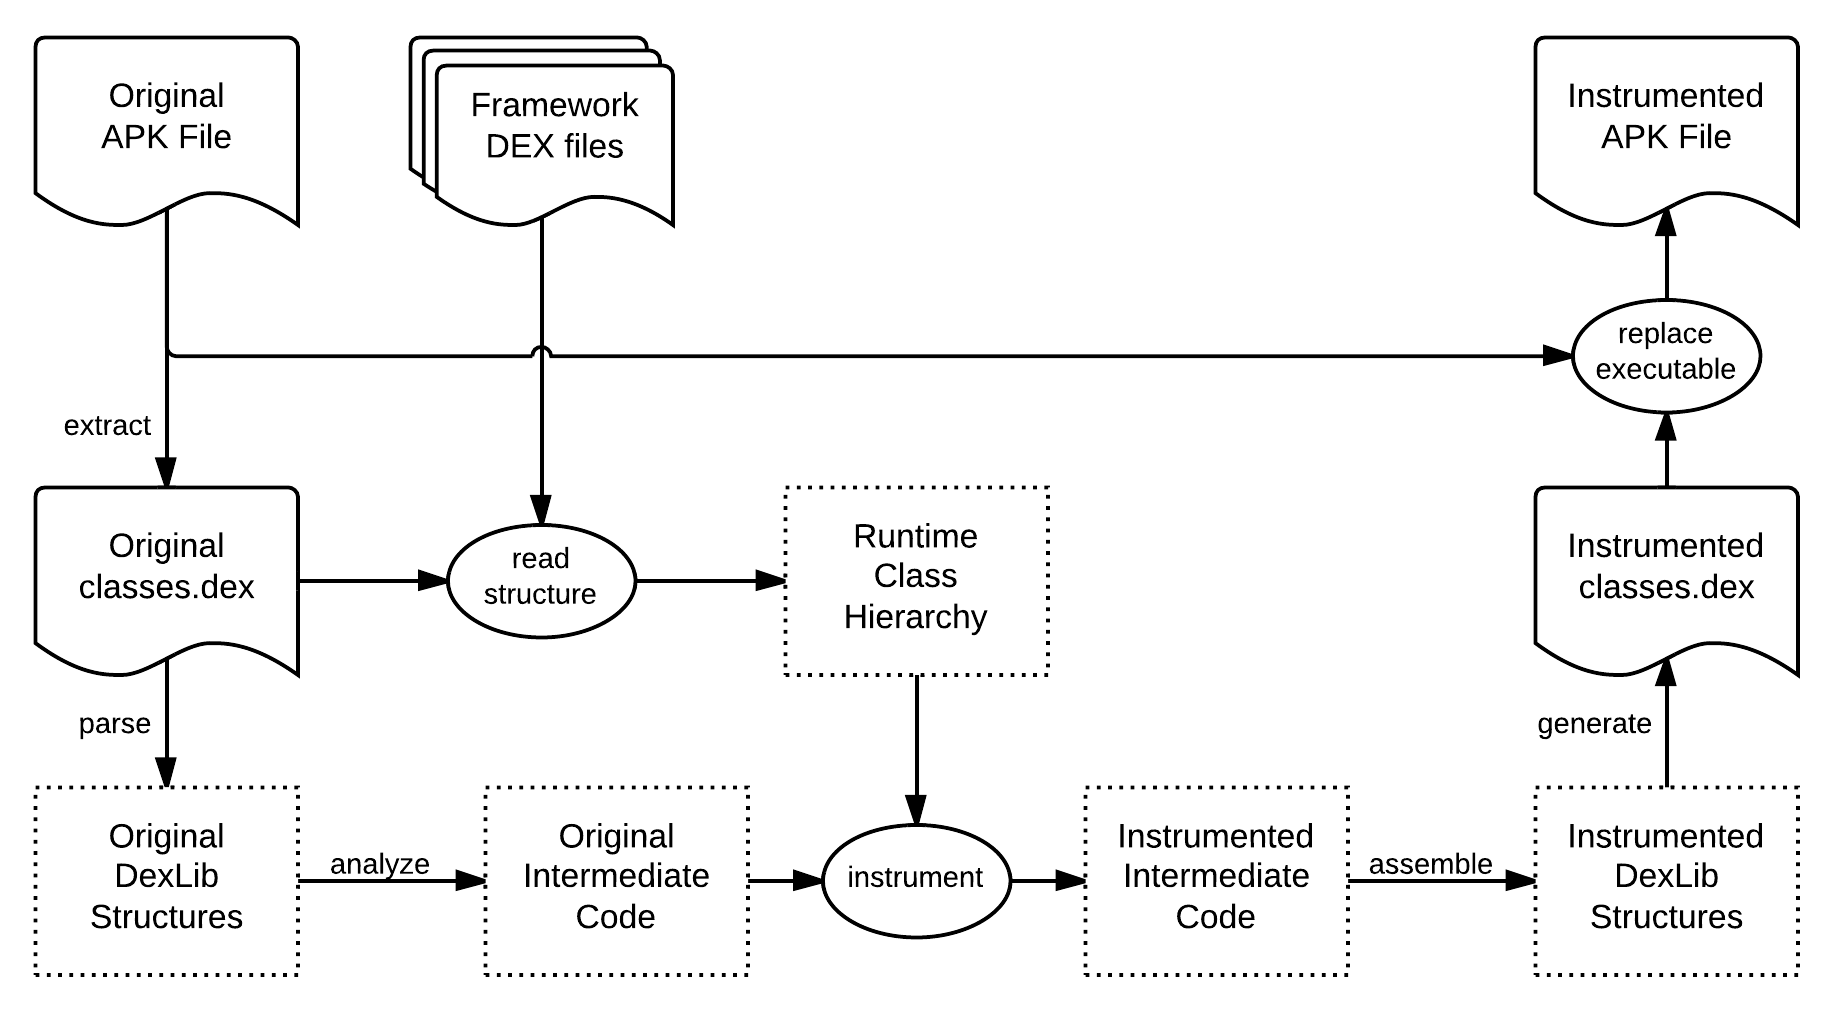
\includegraphics[width=\textwidth]{figs/fig_implementation_overview.png}
	}
	\caption{Schematic diagram of APK instrumentation by Dexter}
	\label{fig:Implementation_Overview}
\end{figure}

The Preparation chapter explained the principles of taint analysis and proposed suitable instrumentation that will carry it out. This part of the dissertation will describe how applications are parsed, additional code inserted, and a new executable generated, a process which will encompass many aspects of compilation. We will also see that more than just a single APK is necessary to reason about the outcomes of dynamic dispatch, and will therefore build a complete picture of the runtime framework. Schematic diagram in Figure~\ref{fig:Implementation_Overview} shows an overview of the individual stages.

\section{Intermediate Representation}

Dexter accesses the content of Dalvik executable DEX files through the low-level API of DexLib. The bytecode and the overall structure of DEX files were designed so that they could be directly mapped to memory and the code executed efficiently, which makes direct instrumentation nearly impossible as even the smallest modification breaks a multitude of pointers and offsets carefully generated by the JVM-Dalvik conversion tool.

Based on the nature of instrumentation introduced earlier, it would be convenient to represent bytecode of individual methods in a way that constraints would not get broken when:
\begin{enumerate}[(i)]
\item new instructions are inserted,
\item extra registers are needed,
\item register identifiers do not fit the addressing limits of instructions,
\item different variants of instructions are used, and
\item try blocks overlap.
\end{enumerate}
Instrumentation will also necessarily introduce new constants and classes, and so Dexter converts the whole executable into its own intermediate representation (IR) and later converts it back to the DexLib format.

\subsection{File Structure}

The logical organization of DEX creates a simple hierarchical arrangement, where the root contains a list of defined classes, those in turn link to methods and fields, etc. DexLib of course implements such a data structure but it could not be utilized since it is not flexible enough for the purposes of Dexter. An equivalent representation was therefore built with ease of element addition in mind.

% The only part of the file that currently cannot be modified are the values of annotations, simply because this feature was not needed. Values of existing annotations are copied over, but only annotations without values can be added.

\subsection{Executable Code}

Method bytecode is stored as a stream of instructions addressed via relative offsets. To support the modifications listed previously Dexter represents bytecode as a list of \emph{code elements}. These are mostly equivalent to instructions but can be interleaved with special markers at positions referencing the offsets in the original DEX file.

\subsubsection{Instructions}

Intermediate instructions group together Dalvik instructions with identical instrumentation. They use intermediate register object references and links to code markers in order to overcome space limits of register identifiers and address offsets, and likewise replace pointers to type information and constants with references to the respective intermediate objects. They also split Dalvik opcodes into semantic equivalence classes and hence allow for conversion between instruction variants.

The instruction interface specifies a list of methods that provide information about them to algorithms working with the bytecode. For instance, these are lists of registers read from and written to, or argument and result types.

\subsubsection{Markers}

Markers specify points inside the bytecode that can be referred to either by instructions or by try-block definitions. Supported markers are:
\begin{itemize}
\item \textbf{labels} \\
Labels mark the targets of jumping and branching instructions. They do not carry any additional information.
\item \textbf{try/catch blocks} \\
Try blocks in DEX are stored separately from the bytecode, and defined as non-overlapping intervals of instructions, which we replace with linked \verb$TryBlockStart$ and \verb$TryBlockEnd$ markers. Each block supplies a list of class type and address pairs that represent its exception handlers. \verb$Catch$ markers are inserted at these points and the list is stored in the start marker. Blocks can also specify an optimized \emph{catch-all} handler used when the exception type does not match any of those on the list.
\item \textbf{method start} \\
\verb$CodeStart$ is a marker inserted at the beginning of each method and used as a reference point for some instrumentation rules.
\end{itemize}

By using markers inside the code, both absolute and relative addresses of these points can be recomputed at the assembly stage, and inserting extra instructions into the code or replacing existing instructions with their different-sized variants does not break any relations.

\subsubsection{Macros}
\label{section:Code_Macros}

Macros provide a way of grouping several instructions into one code element. They were introduced because method calls in Dalvik consist of two separate instructions: an invocation that jumps into the called method, and an optional \verb$move-result$ instruction that stores the returned value into a given register. But since the latter does not contain information about the call, they cannot be instrumented separately. Method calls are therefore replaced with macros before instrumentation begins and expanded afterwards. The same approach is necessary for the \verb$filled-new-array$ instruction.

At the same time, macros are used as inline functions that simplify implementation of some instrumentation rules. We already saw an example of the \verb$taint-get$ macro which expands to:
	\centerbox{
		\asm{invoke-static TaintMap.get(vObject)} \\
		\asm{move-result vResult}
	}
Similar macros were created for common operations like debug logging.

\subsection{Generation Process}

The conversion of the input APK file into intermediate representation is mostly trivial. It is the vast number of DEX elements that need to be supported which makes it a tedious task. 

Given the APK, DexLib extracts the executable and parses it. The data structure it produces is recursively traversed and IR nodes generated from the definitions inside. Encountered pointers are followed into the constant pools of type identifiers, annotations, etc.\ to store data directly in the nodes. During bytecode conversion, introduced markers are stored separately at first and inserted between the instructions once the full instruction list has been created.

% \subsection{Parameter Registers}
% \label{section:Code_ParamRegMapping}

% A very first code modification is also applied at this stage. It later simplifies the process of register allocation by removing one of the constraints the algorithm needs to satisfy, which comes from the fact that every Dalvik method with parameters accesses them through a set of virtual registers with identifiers at the end of the register spectrum it allocates, e.g.\ a method with seven registers and three parameters accesses them through registers \verb$v4$, \verb$v5$ and \verb$v6$ until it overwrites their values. 

% Dexter deals with this by creating a set of registers only for the parameters, inserting \verb$move$ instructions at the beginning of the method to copy the values into the correct registers used in the bytecode, and later explicitly allocating these at the end of the spectrum. This way, register allocation can assign identifiers to the regular registers regardless of this requirement.

\section{Runtime Class Hierarchy}

Section~\ref{section:TaintPropagation_DestDecision} described why it is necessary to be able to argue about the nature of method call destinations and how in most cases analysis of the full class hierarchy can do this statically. Having this data is useful in other situations as well. For example, Listing~\ref{listing:Sink_ApacheHTTPClient_CanBeApplied} was taken from a method that returns \verb$true$ iff the given method call should be instrumented as an Apache HTTP Client sink. As you can see on the highlighted line, it relies on knowing whether the referenced class, probably external, implements the \verb$HttpClient$ interface, and this is the type of information that class hierarchy can provide.

\begin{figure}[h]
	\centering
	\begin{tabular}{c}
	\begin{lstlisting}
val callType = insnInvoke.getCallType();
val invokedClass = insnInvoke.getClassType();
val invokedMethodName = insnInvoke.getMethodName();
val typeHttpClient = DexClassType.parse("Lorg/apache/http/client/HttpClient;", 
                                        parsingCache);

return invokedMethodName.equals("execute") &&
       (
         (
           callType == Opcode_Invoke.Interface && 
           invokedClass.equals(typeHttpClient)
         ) || (
           (callType == Opcode_Invoke.Virtual || 
           	callType == Opcode_Invoke.Super) && 
           `\lsthl{classHierarchy.implementsInterface(invokedClass, typeHttpClient)}`
         )
       );
	\end{lstlisting}
	\end{tabular}
	\begin{lstlisting}[caption={Code that decides whether a method call given by instruction in \texttt{insnInvoke} should be instrumented as an Apache HTTP Client sink.},
	                   label={listing:Sink_ApacheHTTPClient_CanBeApplied}]
	\end{lstlisting}
\end{figure}

As was already mentioned, the hierarchy provides a \emph{complete} picture of the environment the application is executed in, and hence building it obviously requires obtaining class definitions of the runtime framework. Since the API changes with every new release of Android, Dexter does not ship with any particular version and expects the user to provide a compatible set with the application. With access to the device the APK was downloaded from, one can retrieve these files in DEX form from the \verb$/system/framework$ folder, or alternatively provide a compatible \emph{android.jar} file, which applications are compiled against, from the SDK. 

The data structure used for its representation is again a standard rooted tree. Compared to the IR, it holds far less information about its nodes, but spans across the whole runtime environment. Dexter generates it by scanning the DEX and JAR files using DexLib and BCEL\weblink{https://commons.apache.org/proper/commons-bcel/} respectively. Once data are collected, nodes are linked accordingly, and overall consistency is checked.

It is worth pointing out that array types are implicitly defined as classes extending \verb$Object$, i.e.\ they inherit methods like \verb$equals$ and \verb$hashCode$, and method calls can be performed on their instances. As there is no mechanism for extending their interface or overriding the inherited methods, class hierarchy simply treats them as the \verb$Object$ class.

\section{Instrumentation}

Once the executable is parsed and converted, the modifications laid out in the Preparation chapter can be applied on it. This is when all the effort put into designing and generating the IR truly pays off because the source code of instrumentation becomes simple and elegant. 

Every node of the IR is responsible for instrumenting itself, so for example a node representing a primitive internal field creates a new field of type \verb$int$ to hold its taint tag, and gives it a name that will not be in conflict with other fields in the class. Shared data, like these names of taint fields, are stored inside an object that the nodes pass around.

\subsection{Bytecode Instrumentation}

Method body IR nodes generate the analysis-performing instrumentation we are after, and place these new instructions into the code. Implementation of the generators exactly follows the principles of taint propagation explained in section~\ref{section:DataFlowAnalysis} and therefore will not be discussed further. Likewise, the node is responsible for inserting the taint register initialization we saw in section~\ref{section:TaintPropagation_MethodCalls_Internal} at the beginning of the instruction list.

However, the instrumented code might not be valid because instructions which throw exceptions wrap themselves in a try block, like we saw in Figure~\ref{figure:TaintPropagation_ThrowingInstructions}. Had some of these already been in one, the code would now contain two nested try blocks which is an illegal construct. To keep the instrumentation rules simple, we let instructions generate such code and fix it afterwards.

% \begin{figure}[h]
% 	\centering
% 	\begin{minipage}{0.140\textwidth}
% 	\begin{footnotesize}
% 		\asm{TRY\_START\_1} \\
% 		\asm{...} \\
% 		\asm{TRY\_START\_2} \\
% 		\asm{...} \\
% 		\asm{TRY\_END\_2} \\
% 		\asm{...} \\
% 		\asm{TRY\_END\_1}
% 	\end{footnotesize}
% 	\end{minipage}
% 	\begin{minipage}{0.09\textwidth}
% 	\centering
% 	$\Rightarrow$
% 	\end{minipage}
% 	\begin{minipage}{0.150\textwidth}
% 	\begin{footnotesize}
% 		\asm{TRY\_START\_1A} \\
% 		\asm{...} \\
% 		\asm{TRY\_END\_1A} \\
% 		\asm{TRY\_START\_2} \\
% 		\asm{...} \\
% 		\asm{TRY\_END\_2} \\
% 		\asm{TRY\_START\_1B} \\
% 		\asm{...} \\
% 		\asm{TRY\_END\_1B}
% 	\end{footnotesize}
% 	\end{minipage}
% 	\caption{Removing nested try blocks by splitting the outer block.}
% 	\label{figure:Instrumentation_TryBlockSplitting}
% \end{figure}

% The situation and its solution are shown in Figure~\ref{figure:Instrumentation_TryBlockSplitting}. By splitting the outer block into two parts that cover code not covered by the inner block, it becomes valid. Comparing this against the division example referenced earlier, we see that the exception handler ends up inside the second part of the split outer block, and hence re-throwing the exception preserves the original behaviour. However, since Dexter currently does not merge the handler specifications, throwing an exception inside the inner block, originally handled by the outer but now not by the inner, would change it. For this reason, catch-all handlers are used by the instrumentation rules by default. 

\label{section:Code_MethodEntering}

\subsection{Auxiliary Classes}

While the majority of inserted code is generated based on the content of the file, a small part of it is always the same. This common code includes:
\begin{inparaenum}[(i)]
\item the object taint map,
\item the global array and variable for internal method call taint propagation,
\item internality-marking annotations,
\item taint flag constants, and
\item methods analyzing arguments of source API calls.
\end{inparaenum}

These classes could be generated in the same way as the rest of the instrumentation, directly as intermediate code, but for clarity they were written in regular Java. Their source files are compiled using the standard toolchain into a single DEX file that is distributed with Dexter. During instrumentation, this file is converted into IR and the two data structures are merged, effectively statically linking the two files, It is ensured the names of classes do not conflict.

\subsection{Object Taint Map}
\label{section:Code_ObjectTaintMap}

Preparation introduced the idea of a global hash table serving as runtime taint tag storage for objects, and we mentioned above that it is one of the auxiliary classes written in Java and linked in. This section will explain the details and complications of its design.

Na\"{\i}ve usage of the standard \verb$HashMap$ class will immediately fail because storing references to tainted objects in the table prevents their garbage collection. It is therefore necessary to build our hash table on the concept of \emph{weak references} which solve this problem. 

Unfortunately, the standard \verb$WeakHashMap$ implementation calls the \verb$hashCode$ method of given object to determine the slot its entry should be in, and the \verb$equals$ method to compare it against other objects in the linked list of entries in that slot. Calling their default implementations does not have any side effects but they can overridden, and so insertion of the \verb$taint-get$ and \verb$taint-set$ macros could introduce method calls that were not present in the original application and potentially change its behaviour. At the same time, one can easily make all objects look equivalent which would uncontrollably spread taint. And lastly, the class does not account for the fact that these methods could throw exceptions. For all these reasons, a safe version of \verb$WeakHashMap$, which would not call any of the object's methods, had to be implemented. 

Removing the call to \verb$equals$ is trivial, simply by using the reference equality operator \verb$==$ instead. The \verb$obj.hashCode()$ call, on the other hand, was replaced by \verb$obj.getClass().hashCode()$. The \verb$getClass$ method cannot be overridden as it is declared \verb$final$, and it returns an instance of class \verb$Class$ which represents the type of \verb$obj$. These \verb$Class$ objects are automatically generated by the virtual machine when classes are loaded, and so \verb$equals$ cannot be overridden and always uses the original implementation which returns its address in the memory. Unfortunately, this means that all instances of one class type will generate the same hash code and will be stored in the same slot. If this ever proved to be a performance bottleneck, native code could be used to return addresses of individual objects with the cost of reducing portability of the solution. 

In its current implementation, the hash table is initialized with 1024 slots and does not support dynamic resizing. It exploits temporal locality by moving entries to the beginning of their respective linked lists whenever they are accessed, and deletes garbage collected entries as it encounters them. Methods are declared \verb$public static$ so that they can be invoked from any place in the application.

\section{Reassembling}

In the context of Dexter, reassembling is the process of converting IR back to DexLib data structures. Conversion of most nodes is straightforward as DexLib automatically assembles constant pools, class/method/field definitions, etc., and replaces references to them with numerical pointers. 

But it is up to Dexter to generate Dalvik bytecode with register identifiers and jumping offsets that fit the space limits of its instructions. Instrumentation more than doubled the number of used intermediate registers, and the offsets increased as instructions were inserted between the jumping instructions and their targets. For instructions that can only carry 4-bit register identifiers or offsets, this becomes a problem.

The following sections will explain how intermediate registers are assigned new identifiers that fit these constraints. Since offset computation relies on the knowledge of the register identifiers, it is discussed at the end.

Similar procedures form the core of the compilation process of any programming language, and therefore a full-fledged compiler capable of generating Dalvik bytecode from Dexter IR had to be implemented. The compiler was built according to~\cite{Appel:2003:MCI:599718}, and hence the details of generic algorithms will be omitted and focus will be put on the specifics of Dalvik. Building a compiler is itself a task difficult to achieve within the given project time frame. On that account, basic algorithms with simple heuristics were selected, regardless of the performance of the generated code or their own time complexity.

\subsection{Generic Register Allocation}

Register allocation is an optimization problem of assigning a large number of source code variables to a small number of CPU registers. Same register can be used to hold the value of multiple variables as long as the variables are not \emph{live} at the same time, i.e.\ the intervals between storing a value and the last point of reading it back do not overlap. 

If a solution cannot be found, memory storage is created for some of the variables and load/store instructions moving the value to/from designated temporary registers are inserted, so that the algorithm can be restarted with reduced number of variables held in CPU registers at the same time. This is called \emph{variable spilling}.

\subsubsection{Allocation by Graph Colouring}

A compiler reduces the register allocation to the isomorphic problem of graph colouring, which is proven to be NP-complete, and solves it using a heuristic that balances time complexity of the algorithm with quality of the generated code. 

The graph in question is called a Clash Graph (CG). Its nodes represent variables, and two nodes are connected by an edge iff the two respective variables cannot be allocated to the same register. If this graph can be coloured with a number of colours less than or equal to the number of available CPU registers, a solution has been found. 

\begin{figure}
	\centerline{	
		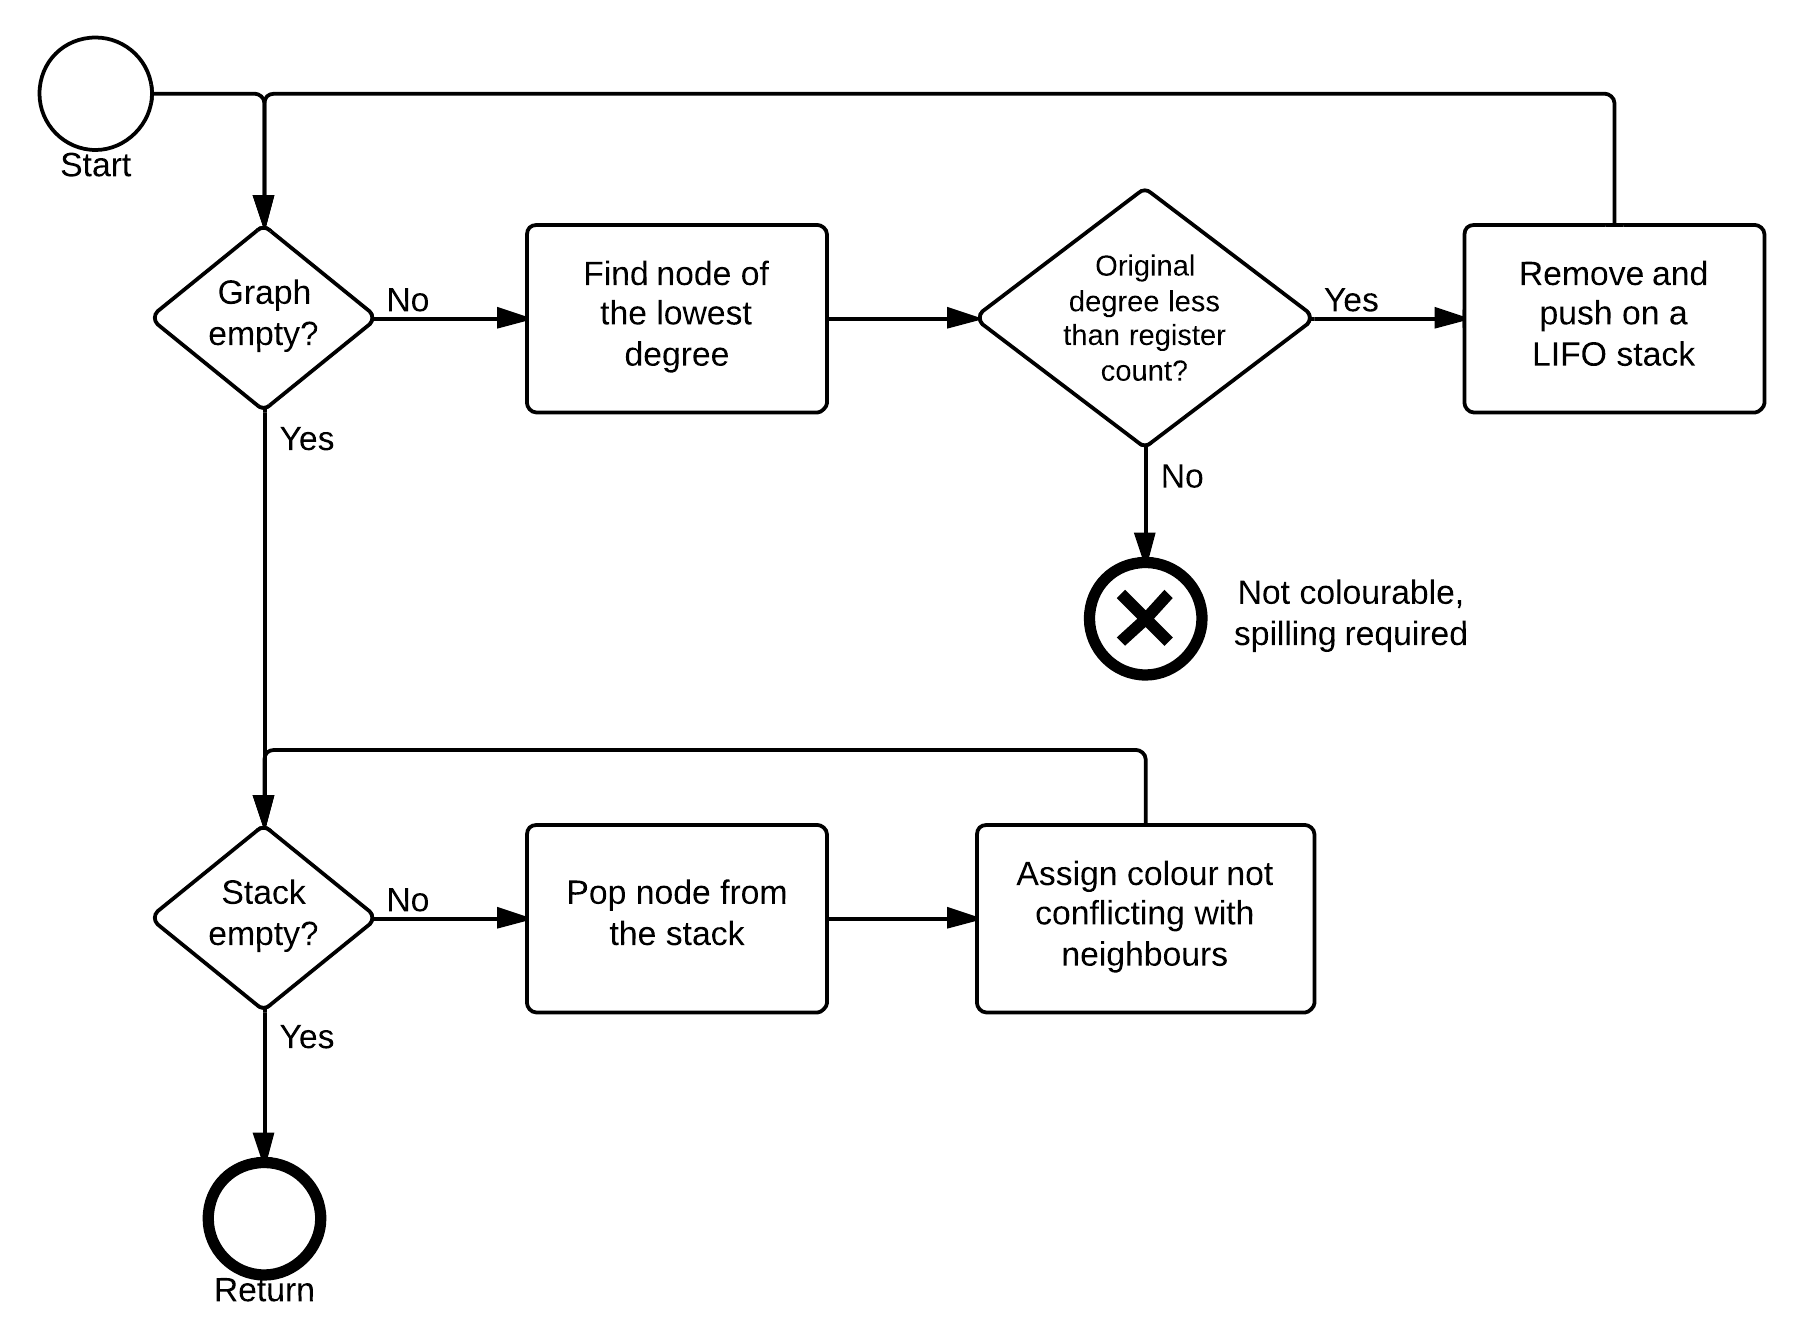
\includegraphics[width=0.9\textwidth]{figs/fig_implementation_gc.png}
	}
	\caption{Flow chart of commonly used greedy graph-colouring heuristic.}
	\label{fig:Implementation_GraphColouring}
\end{figure}

Figure~\ref{fig:Implementation_GraphColouring} shows a commonly used greedy graph-colouring algorithm, which Dexter adopts with slight modifications explained later. The heuristic colours the nodes, ordered by the number of constraints, starting with the most constrained one and always picking a colour not taken by the neighbours. It runs in linear time and usually yields satisfactory results.

\subsubsection{Building a Clash Graph}

The CG is built by comparing the liveness of individual variables, which can be established by performing so-called Live Variable Analysis (LVA) on the Control Flow Graph (CFG) of the method code. Two variables simultaneously live at any point should be connected by an edge.

The CFG is a graph with nodes representing maximal sequences of non-jumping instructions, called basic blocks, and nodes $A$ and $B$ being connected by a directed edge iff the execution of last instruction in $A$ can be followed by the execution of first instruction in $B$. For example, an \verb$if$ instruction always ends its basic block as it can either proceed to the next instruction or jump to a marker. Two special nodes, \verb$START$ and \verb$EXIT$, represent the entry and exit points of the method and are connected accordingly.

The principle of CFG generation is not complicated. Code elements specify whether they start/end basic block (labels, \verb$if$), or exit the method (\verb$return$), and also provide the complete list of their successors. One linear pass over the instruction list is then sufficient to split it into blocks, and one more iteration over the blocks enough to create the edges.

Crucial property of the CFG is its completeness, or else incorrect liveness intervals can be produced and clashes missed. A lot of effort was therefore invested into reading the Dalvik documentation to ensure the properties of code elements correctly reflect all aspects of the execution semantics. This sometimes requires a simple code analysis, like finding the catch block the program will jump to if an exception of given type is thrown by a particular instruction. 

\begin{figure}
	\centerline{	
		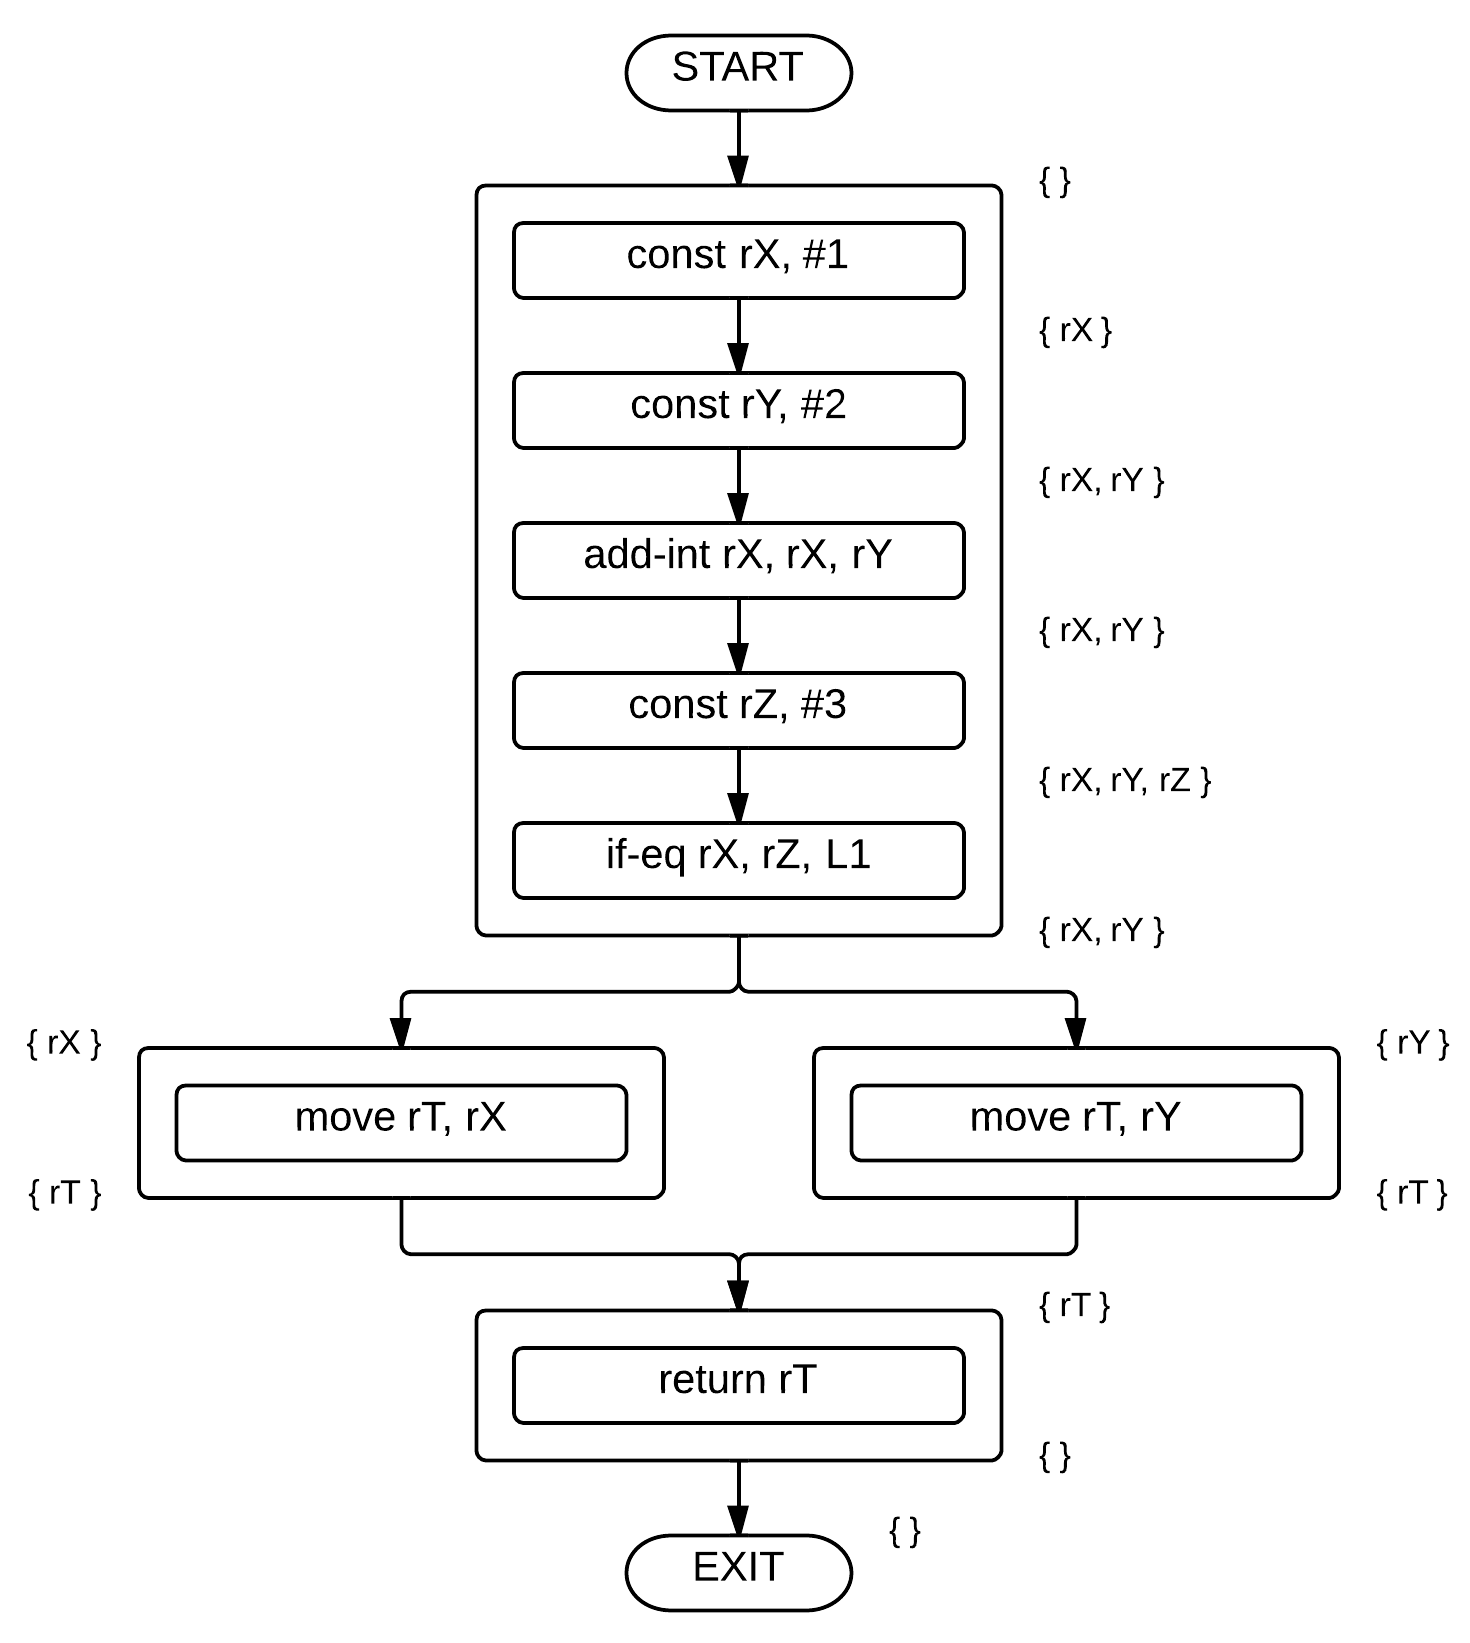
\includegraphics[height=0.42\textheight]{figs/fig_implementation_lva.png}
	}
	\caption{Example of Live Variable Analysis performed on a simple program represented as a Control Flow Graph. Live variables at each execution point are in brackets.}
	\label{fig:Implementation_LVA}
\end{figure}

The live variable analysis is based on the idea of propagating information about variables being read from to preceeding instructions, so that it is known which values might be needed in the future for each position in the code. A loop iterates through the instructions, always combining the lists of variables provided by its successors, removing variables it writes to and adding those it reads from. Being defined as least fixed point, the loop carries on until no more changes are made. An example is shown in Figure~\ref{fig:Implementation_LVA}.

Each variable list generated by LVA then specifies variables that cannot be allocated to the same register because their values are simultaneously waiting to be read. An edge in clash graph is therefore generated for each pair of variables that appear together in some variable list.

\subsection{Dalvik Register Allocation}

It is easy to see how the generic register allocation fits into the reassembling procedure in Dexter. Register objects inside intermediate code can be thought of as untyped variables, and these need to be mapped on Dalvik's virtual registers. But due to constraints imposed on the identifiers, the graph-colouring heuristic requires small alterations.

\subsubsection{Register-Addressing Limits}

The first distinction is that colouring is not limited to a fixed number of colours, since Dalvik instruction formats differ in the amount of space available to store register identifiers. Hence each node has its own upper identifier limit given by bit representations of the least optimized variants of instructions that use the corresponding intermediate register.

The way the heuristic chooses colours is changed to reflect this. So as not to pollute smaller ranges, colours are preferentially picked from the higher parts of the spectrum. For instance, for node restricted to the \mbox{0-255} range, a colour in \mbox{16-255} will be sought first.

\subsubsection{Consecutive-Identifier Constraints}

The algorithm also needs to deal with Dalvik instructions which reference registers implicitly. The reason why wide register pairs need to be formed by two adjoined virtual registers is that instructions always store only the identifier of the first one. The same concept applies to \verb$/range$ variants of \verb$invoke$ instructions which use an interval of registers as method arguments by specifying the first identifier and the length of the interval.

IR instructions reference all intermediate registers explicitly and provide their allocation constraints. These are collected, checked for conflict, and so-called \emph{node runs} built. These are maximal sequences of CG nodes required to be assigned consecutive identifiers. 

The order generator still picks the node of the lowest degree but now finds the node run it belongs to, pushes the run on the stack and removes all its nodes from the graph, defining an order of colouring runs instead of individual nodes. The colouring loop pops a run, finds a non-conflicting colour for its first node and checks whether the other nodes can be assigned the following colours. This is repeated until either a valid colouring of run is found or all initial node colours have been tried.

\subsubsection{Variable Spilling}

We already mentioned that if a colouring cannot be found the compiler spills some variables into external memory so that fewer variables need to be allocated to registers. However, this concept does not directly apply to Dalvik since it only provides the notion of 65k virtual registers, some mapped to physical registers and rest stored on the stack. The equivalent operation is therefore a transformation of the IR code which creates new temporary registers and inserts \verb$move$ instructions before and after every instruction that uses the spilled ones. Note that we always need to spill whole node runs because of consecutive-identifier constraints.

\begin{figure}
\subfigure{
	\centering
	\begin{minipage}{0.325\textwidth}
	\begin{footnotesize}
		\asm{int-to-long rA1 | rA2, rB} \\
		\asm{...} \\
		\asm{int-to-long rA2 | rA3, rC}
	\end{footnotesize}
	\end{minipage}
	\begin{minipage}{0.09\textwidth}
	\centering
	$\Rightarrow$
	\end{minipage}
	\begin{minipage}{0.465\textwidth}
	\begin{footnotesize}
		\asm{move-wide pTemp1 | pTemp2, rA1 | rA2} \\
		\asm{int-to-long pTemp1 | pTemp2, rB} \\
		\asm{move-wide rA1 | rA2, pTemp1 | pTemp2} \\
		\asm{...} \\
		\asm{move-wide pTemp3 | pTemp4, rA2 | rA3} \\
		\asm{int-to-long pTemp3 | pTemp4, rC} \\
		\asm{move-wide rA2 | rA3, pTemp3 | pTemp4}
	\end{footnotesize}
	\end{minipage}
}

\subfigure{
	\centering
	\begin{minipage}{0.325\textwidth}
	\begin{footnotesize}
	\begin{tabular}{|c|c|}
		\firsthline
		\textbf{Variable} & \textbf{Constraint} \\
		\hline
		\texttt{rA1} & 4-bit identifier \\
		\texttt{rA2} & following \texttt{rA1} \\
		\texttt{rA2} & 4-bit identifier \\
		\texttt{rA3} & following \texttt{rA2} \\
		\lasthline
	\end{tabular}
	\end{footnotesize}
	\end{minipage}
	\begin{minipage}{0.09\textwidth}
	\centering
	$\Rightarrow$
	\end{minipage}
	\begin{minipage}{0.35\textwidth}
	\begin{footnotesize}
	\begin{tabular}{|c|c|}
		\firsthline
		\textbf{Variable} & \textbf{Constraint} \\
		\hline
		\texttt{rA1} & 16-bit identifier \\
		\texttt{rA2} & following \texttt{rA1} \\
		\texttt{rA2} & 16-bit identifier \\
		\texttt{rA3} & following \texttt{rA2} \\
		\texttt{pTemp1} & 4-bit identifier \\
		\texttt{pTemp2} & following \texttt{pTemp1} \\
		\texttt{pTemp3} & 4-bit identifier \\
		\texttt{pTemp4} & following \texttt{pTemp3} \\
		\lasthline
	\end{tabular}
	\end{footnotesize}
	\end{minipage}
}

	\caption{Example of variable spilling transformation and change in constraints.}
	\label{figure:Reassembling_VariableSpilling}
\end{figure}

The idea is demonstrated on an example in Figure~\ref{figure:Reassembling_VariableSpilling}. In the original form we see a three-element node run with its first two nodes confined to the 4-bit range. On the other hand, by spilling the run these three nodes can be stored in the full 16-bit range and we get two two-element runs in the 4-bit range which can be allocated the same identifiers as their liveness intervals do not overlap.

Choosing the optimal subset of variables to spill is an entirely different topic, so for the sake of simplicity, a random node run is chosen from the range that filled up and caused the colouring to fail, and colouring restarted.

However, not all node runs can be spilled this way because \texttt{move} instructions are typed, distinguishing between single-/double-width primitives and objects, and this is checked by the preload verifier. Types are decidable from semantics of the transformed instruction, with the exception of \emph{if (not) equal to (zero)} statements which can compare both single-width primitives and references. Spilling node runs appearing in these would therefore require more sophisticated type inference.

\subsection{Static Single-Assignment Form}

The described algorithm successfully allocates most methods, yet it is not uncommon for an application to contain one on which it fails. Through a mixture of wide register operations and \texttt{/range} method calls, such code typically defines an unspillable node run of 20 or even 30 intermediate registers, completely polluting the 4-bit range, leaving no room for the taint registers, and consequently preventing Dexter from generating the instrumented executable. Static Single-Assignment (SSA) form, a result of another intermediate code transformation, breaks node runs into the smallest possible pieces.

SSA form is defined as one where each variable is written to only once, and is created by renaming variables. Looking back on the spilling example in Figure~\ref{figure:Reassembling_VariableSpilling}, both of the instructions wrote to \texttt{rA2} which created the three-element run. By renaming the variables we get two smaller, more easily allocatable runs \texttt{{[}rA1$_1$, rA2$_1$]} and \texttt{{[}rA2$_2$, rA3$_1$]} without changing the behaviour.

\begin{figure}
  \centering
  \subfigure[Original code]{
  	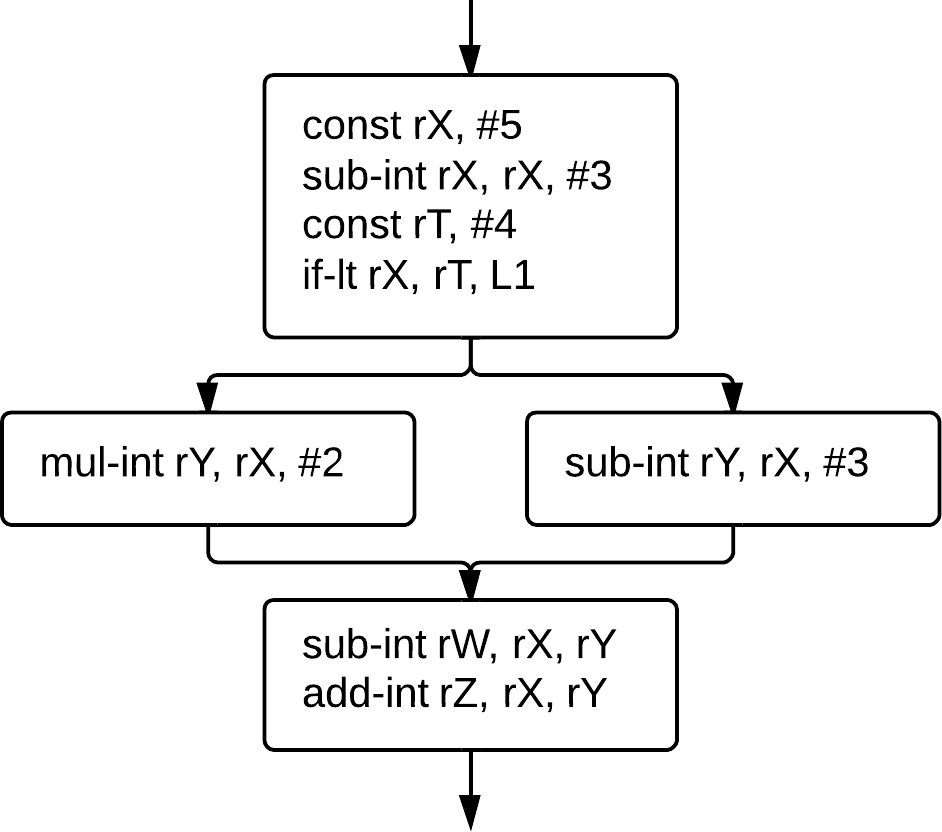
\includegraphics[width=16pc]{figs/fig_implementation_ssa1.png}
  }
  \label{figure:Implementation_SSA1}
  \subfigure[$\Phi$ function inserted]{
  	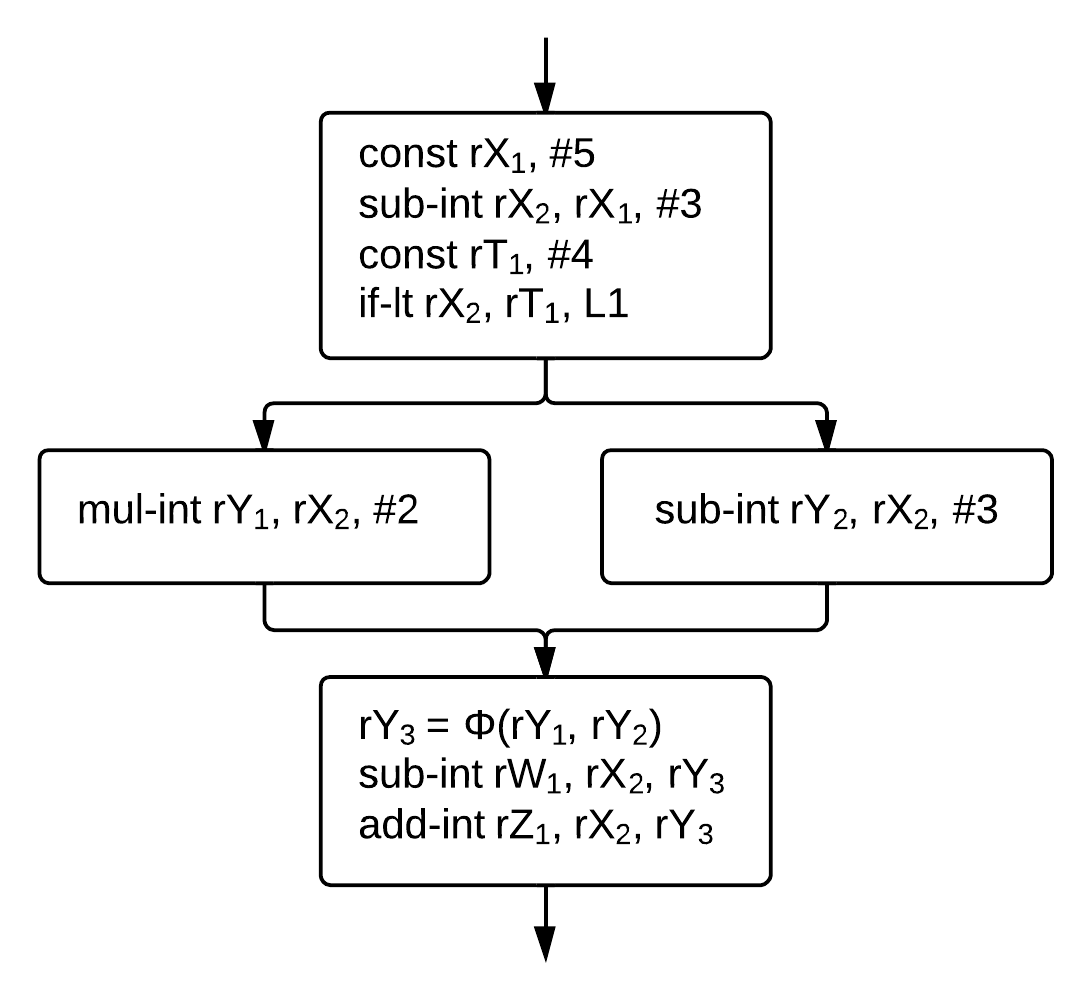
\includegraphics[width=16pc]{figs/fig_implementation_ssa2.png}
  }
  \label{figure:Implementation_SSA2}
  \subfigure[$\Phi$ function converted to \texttt{move} instructions]{
  	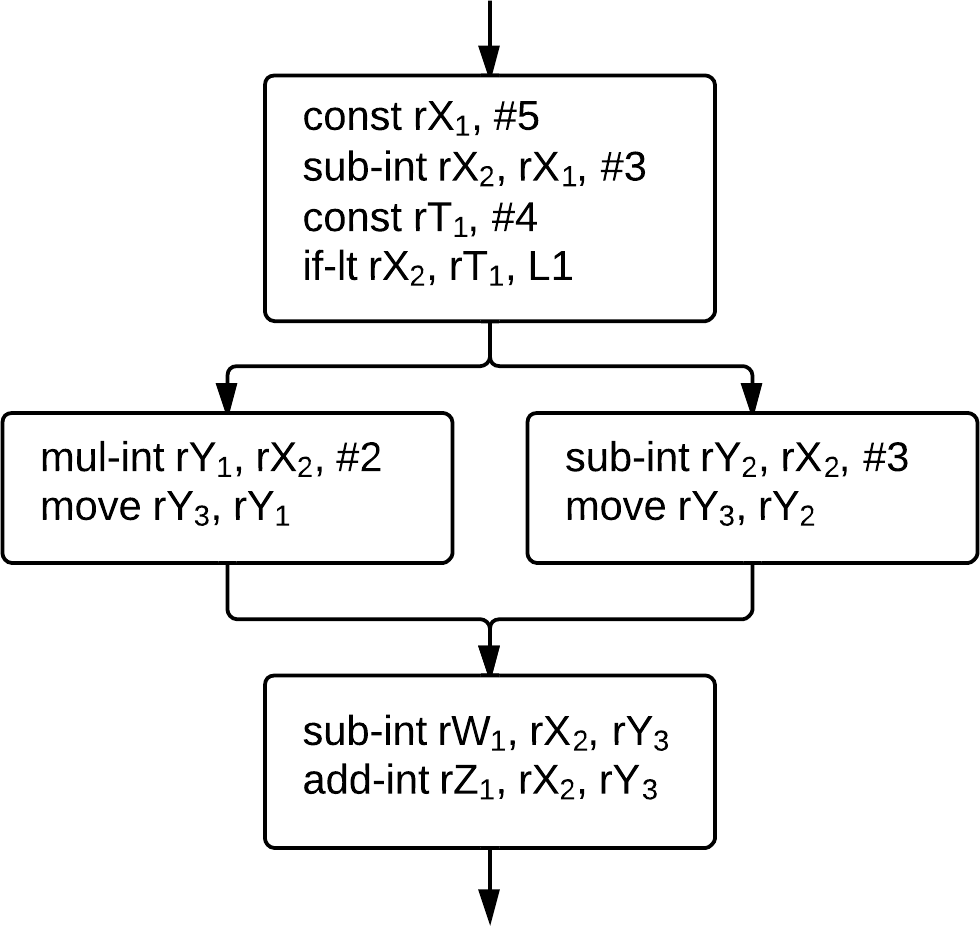
\includegraphics[width=16pc]{figs/fig_implementation_ssa3.png}
  }
  \label{figure:Implementation_SSA3}

  \caption{Example of SSA transformation}
  \label{figure:Implementation_SSA}
\end{figure}

Figure~\ref{figure:Implementation_SSA} shows that the transformation is not as straightforward in the general case. Variable $rY$ is defined in both branches of the \texttt{if} statement, and so renaming these to $rY_1$ and $rY_2$ also requires combining their values into $rY_3$ before referencing them later on. 

Transformation to SSA is done in three steps:
\begin{inparaenum}[(i)]
\item points in CFG where variable definitions meet are identified and $\Phi$ functions combining the values inserted,
\item $\Phi$ functions are converted to \texttt{move}s inside predecessor blocks,
\item redundant \texttt{move}s are removed.
\end{inparaenum}
These rely on further analysis of the code. For instance, the points of definition conflict are found by converting CFG to \emph{Dominator Tree} and performing \emph{Dominance Frontier Analysis} on it~\cite{Appel:2003:MCI:599718}.

The principles behind SSA transformation are not complicated but its implementation for specific platform requires careful adaption, e.g.\ with Dalvik by propagating type information to insert valid \texttt{move}s. The transformation was fully implemented and shown to work on small methods otherwise impossible to allocate, but it would require more time to make it production-ready. Applications presented in Evaluation were instrumented without it.

\subsection{Offset Computation}

Returning to the generation of Dalvik bytecode, intermediate instructions still cannot be asked to produce their Dalvik counterparts as we have not yet computed offsets to the markers they reference. To compute the offsets we need to know the sizes of the Dalvik instructions, and so the problem is solved iteratively.

The algorithm starts by creating a list of sizes initially set to one, passing it together with register allocation to the instructions and letting them generate their most optimized Dalvik variants. Instruction sizes are updated and previous steps repeated until convergence is reached. The algorithm is guaranteed to terminate since instructions can only grow in size because offsets overflowling the space reserved in the current variant forces generation of a bigger one, or causes failure if such variant does not exist.

\begin{figure}[t]
	\centering
	\begin{minipage}{0.28\textwidth}
	\begin{footnotesize}
	\begin{tabular}{l}
		\asm{if-eq rA, rB, LTarget} \\
		\asm{...} \\
		\asm{LTarget:}
	\end{tabular}
	\end{footnotesize}
	\end{minipage}
	\begin{minipage}{0.09\textwidth}
	\centering
	$\Rightarrow$
	\end{minipage}
	\begin{minipage}{0.25\textwidth}
	\begin{footnotesize}
	\begin{tabular}{l}
		\asm{if-eq rA, rB, LJump} \\
		\asmExtra{goto LSuccessor~~~~} \\
		\asmExtra{LJump:~~~~~~~~~~~~~} \\
		\asmExtra{goto LTarget~~~~~~~} \\
		\asmExtra{LSuccessor:~~~~~~~~} \\
		\asm{...} \\
		\asm{LTarget:}
	\end{tabular}
	\end{footnotesize}
	\end{minipage}
	\caption{Example of an \texttt{if} instruction fixing unreachable target.}
	\label{figure:Reassembling_FixLongJump}
\end{figure}

If it fails, the jumping instruction is asked to instrument itself in order to fix this problem. As one can see in Figure~\ref{figure:Reassembling_FixLongJump}, \verb$goto$ is used to do the jump for the instruction because its least optimized variant can store safe 32-bit offsets.

\section{APK Repackaging}

With DexLib having generated the final executable, Dexter has to substitute it for the original \emph{classes.dex} inside the APK. 

Since APKs are mere ZIP files, the Zip4j\weblink{http://www.lingala.net/zip4j/} library was used to replace the file and also to remove the \verb$META-INF$ folder containing the original (now invalid) digital signature. The last step of the lengthy process of instrumentation is therefore calling tools from the \emph{Java Development Kit} to generate a random key and sign the package with it.

\cleardoublepage
\chapter{Evaluation}

\subsection{User Interaction}

When imminent data leakage is identified, the instrumented application should ideally display a dialog, providing information about the event and offering either to continue or to terminate itself. However, the standard Android programming model does not provide any form of execution pausing mechanism which could be used to show a modal window without the application being killed by the operating system for non-responsiveness. In addition, background-running threads are not even allowed access to the UI. Implementation of this feature therefore proved extremely complicated, requiring deeper access to the system message loop, and Dexter currently only prints its warnings into the system log.

focus is on security experts (log is MORE HELPFUL)!!!!

\section{Case Studies}

\subsection{Android/GoneSixty}

Gone in 60 Seconds is a piece of spyware which the author claims was written for educational purposes only. Initially available on the Google Play market, users would download the application and then watch it swiftly send their sensitive data to a remote server immediately after first launch. Even though GoneSixty is virtually harmless and its methods of distribution and data collection unsophisticated, it nicely demonstrates how various data sources are accessed, and also propagates the data to a sink in a nontrivial way. A security report by AVG, with more details on how GoneSixty works, can be found in Appendix~\ref{chapter:Report_Gone60}.

\begin{figure}[t]
	\scriptsize
	\begin{verbatim}
I/ActivityManager(  187): Start proc com.gone603 for activity com.gone603/com.gone60.gone60: 
                          pid=10912 uid=10065 gids={3003}
I/System.out(10912): $ content query: content://com.android.contacts/contacts => 1
I/System.out(10912): $ content query: content://sms => 2
I/System.out(10912): $ browser data => 16
I/System.out(10912): $ content query: content://call_log/calls => 4
I/System.out(10912): $ content query: content://com.android.contacts/data/phones => 1
I/System.out(10912): $! tainted Apache HTTPClient request executed => T=23
	\end{verbatim}
	\caption{Log output generated by the instrumented version of GoneSixty.}
	\label{figure:Evaluation_GoneSixty}
\end{figure}

Manual inspection of the bytecode showed that GoneSixty runs five threads. The first four acquire:
\begin{inparaenum}[(i)]
\item contact list,
\item text messages,
\item recent calls,
\item browser history,
\end{inparaenum}
and store the data into commonly accessible class fields. The fifth thread waits for the other four to finish and combines the data into a single JSON structure first. They are then sent to to a remote server as an HTTP POST request using the Apache client. Output of the instrumented application in Figure~\ref{figure:Evaluation_GoneSixty} shows that Dexter correctly identified access to all four of these sources, successfully propagated the taint tags all the way to the HTTP request execution and printed a leakage warning. 

\subsection{Android/BgServ}

The second analyzed application was infected with the BgServ trojan, which is significantly more dangerous and complex than GoneSixty. Discovered in March 2011, it was inserted into various ordinary applications and then distributed through third party application markets. It runs in the background, sends sensitive data to a remote location and opens a backdoor. The trojan receives orders from a remote server, and sends premium-rate SMS messages or changes Internet connection settings. Appendix~\ref{chapter:Report_BgServ} contains a security report by Symantec with further details. 

\begin{figure}[t]
	\scriptsize
	\begin{verbatim}
I/ActivityManager(  182): Start proc com.virsir.android.chinamobile10086 for activity 
                          com.virsir.android.chinamobile10086/com.mms.bg.ui.FakeLanucherActivity: 
                          pid=712 uid=10058 gids={3003, 1015}
I/System.out(  712): $ system service request: layout_inflater => 0
D/FlurryAgent(  712): Starting new session
I/System.out(  712): $ system service request: location => 8
D/FlurryAgent(  712): Sending report to: http://data.flurry.com/aar.do
I/System.out(  712): $! tainted Apache HTTPClient request executed => T=8
I/System.out(  712): $ system service request: notification => 0
I/System.out(  712): $ system service request: connectivity => 0
I/System.out(  712): $ system service request: wifi => 0
I/System.out(  712): $ content query: content://telephony/carriers/preferapn => 0
I/System.out(  712): $ system service request: phone => 32
I/System.out(  712): $ system service request: wifi => 0
I/System.out(  712): $! tainted Apache HTTPClient request executed => T=32
D/FlurryAgent(  712): Ending session
	\end{verbatim}
	\caption{Partial output generated by the instrumented version of BgServ. Repeated and irrelevant lines were removed.}
	\label{figure:Evaluation_BgServ}
\end{figure}

Unlike GoneSixty, which steals personal data, BgServ is interested in information that can identify the device: phone number, IMEI, version of the system, etc. These are accessed through system service managers and from the output in Figure~\ref{figure:Evaluation_BgServ} we see that Dexter recognized access to location and phone service managers, and that the data are again being leaked via HTTP. This is consistent with findings made by the TaintDroid team, who analyzed it as well.

As one can also see from the output, Bgserv requests access to a few other system services and reads network settings from the database. These are not being tracked at the moment, but support could easily be added. Moreover, the security report mentions that data are written into a temporary file before they are sent to the server. Bytecode inspection revealed that BgServ uses \verb$XmlSerializer$\weblink{https://developer.android.com/reference/org/xmlpull/v1/XmlSerializer.html}, which is currently not a recognized sink, but could be easily added to the Dexter framework.

\subsection{Find\&Call}

Find\&Call is a contact organizer, whose iOS version became known as the first malware for the platform, approved by Apple and distributed through App Store. It also briefly appeared on Google Play before it was removed in July 2012. Find\&Call leaks contact list and phone number data which are used by the server to send spam via text messages that appear to be sent by the user. A blog entry~\cite{report:FindAndCall} by a Kaspersky Lab expert provides more information.

Dexter discovered multiple HTTP requests leaking the contents of the phonebook and user's location. Access to the service providing phone number information was also identified, but tagged data never reached the sink, which might indicate a bug in the implementation of Dexter or they simply were not leaked. Since the application is complex and its bytecode had been obfuscated, further investigation of this by hand was not successful. 

The Dexter output also shows that sensitive data are being shared between application's components (activities) through IPC calls, and that these correctly propagate taint without requiring any extra instrumentation.

\section{Performance Overhead}

The extra work done by taint tracking instructions naturally has a negative effect on the overall performance of the application. Similar systems tend to incur 2-20 times slowdown~\cite{Yin:2007:PCS:1315245.1315261, Chow:2004:UDL:1251375.1251397}, but this is usually acceptable because these techniques are generally used with applications that mostly wait for user's input and perform very little computation. 

The overhead of Dexter's instrumentation was assessed and the results are presented in this section. All experiments were conducted on Google Nexus One running Android 2.3. 

\subsection{Benchmark}

\begin{figure}
	\centerline{
		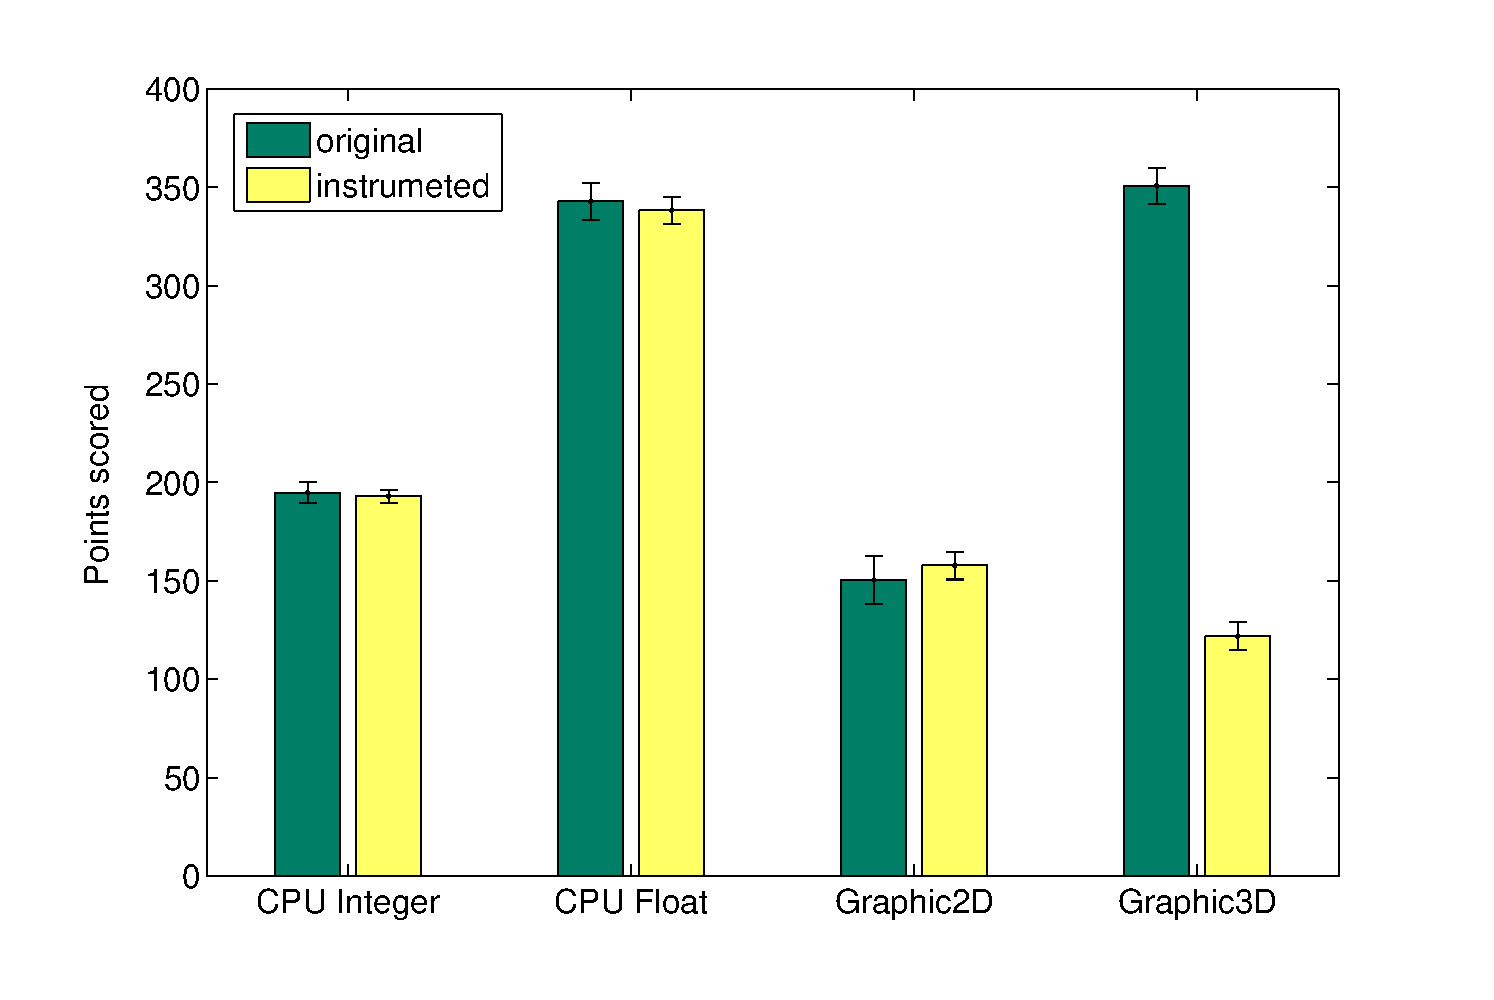
\includegraphics[width=0.7\textwidth]{figs/fig_eval_quickbench.eps}
	}
	\caption{Points scored in QuickBenchmark. Error bars represent interval of one standard deviation. Each version of the application was run 37 times.}
	\label{figure:Evalutaion_QuickBench}
\end{figure}

To measure the overhead of heavily processor-bound computation, a benchmark application was downloaded from the official market, instrumented and results compared with the original. Unfortunately, benchmarks commonly used by the community, like AnTuTu or Quadrant, run their tests in native code which is not instrumented. A lesser known QuickBenchmark therefore had to be chosen instead. Results are summarized in Figure~\ref{figure:Evalutaion_QuickBench}. 

The first two tests simply run a loop in which they perform integer and float computation respectively. Even though for each such instruction, the instrumentation adds an OR of the taint tags, the difference was less than 2\% and well within the margin of error in both cases. The reason probably lies in the fact that the original computation and taint tracking have zero data dependencies between each other, which allows the superscalar CPU to execute them out of order and hence fill pipeline stalls.

The third test draws 2D shapes on the screen, animates them and measures the frame rate. Similarly to the first two, it runs a loop with some floating point computation, but also calls external drawing methods. Since it operates only with primitives, with no dependencies whatsoever, and instrumentation of external calls is cheap, we still do not see a speed drop. On average, the benchmark actually awarded slightly more points to the instrumented version. possibly due to better register allocation, but the results are still within one standard deviation of each other. 

The last test shows how expensive taint tracking can be. The test draws two rotating cubes in 3D with OpenGL, which is roughly equivalent to the 2D test, except each cube is represented as an instance of a cube class. The additional use of expensive internal calls results in a 65\% performance drop.

\subsection{Source Access}

\begin{figure}
	\centerline{	
		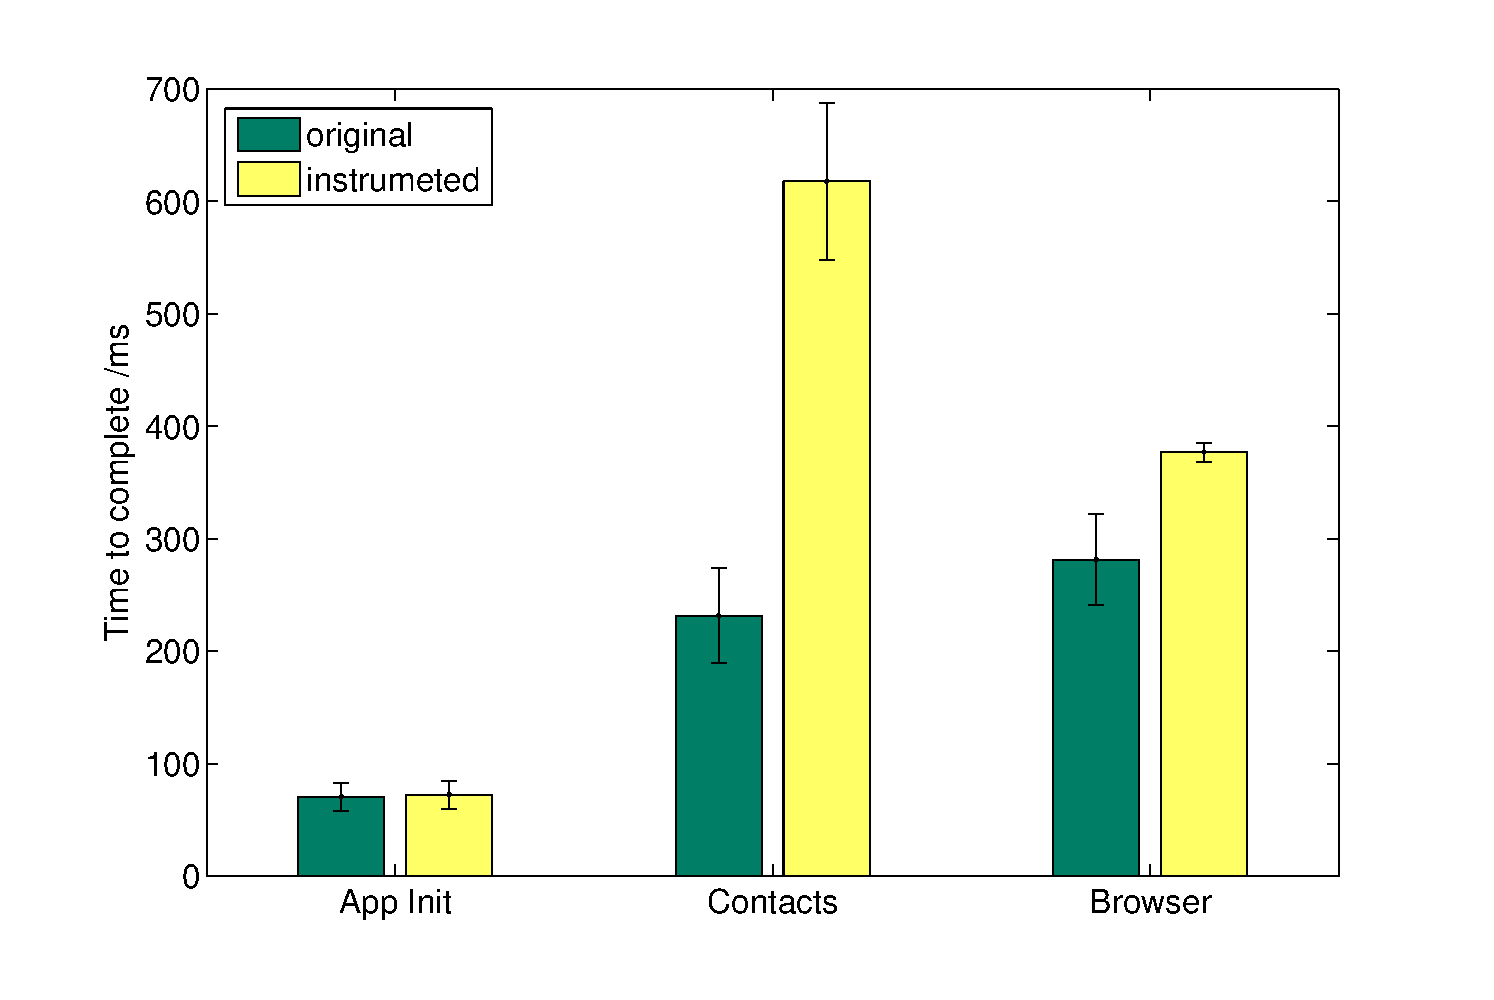
\includegraphics[width=0.7\textwidth]{figs/fig_eval_testappbench.eps}
	}
	\caption{Time taken to initialize the application and access sources. Error bars represent interval of one standard deviation. Each test was executed 100 times.}
	\label{figure:Evalutaion_TestAppBench}
\end{figure}

Since the benchmark works nearly exclusively with primitives and does not access any sensitive data, further experiments were conducted on an in-house testing application. Measured operations are equivalent to those assessed under TaintDroid for comparison. Graph in Figure~\ref{figure:Evalutaion_TestAppBench} shows the results.

Load time of the application was hardly affected by the instrumentation, slowing down from 70ms to 72ms, and exactly matching TaintDroid in performance. 

Reading the phonebook, as shown in Listing~\ref{listing:Source_DatabaseQuery}, saw a significant decrease in performance, taking nearly three times as long. This is partially caused by the analysis of the database query, but mainly by the propagation of taint into returned string objects, which all collide when stored in the object taint map. According to the academic paper, a similar operation on TaintDroid had overhead of eighteen percent. A better global hashmap implementation, as suggested in section~\ref{section:Code_ObjectTaintMap}, is likely to help.

Access time was also measured for the web browsing history, similar to that in Listing~\ref{listing:Source_Browser}. Slowing down by approximately a quarter, the difference is considerably smaller because no string comparisons of the query are carried out, and far fewer strings are tainted as only a single column is read from the results, in contrast to four in the previous test.

\section{Code Bloat}

\begin{figure}
	\centerline{
		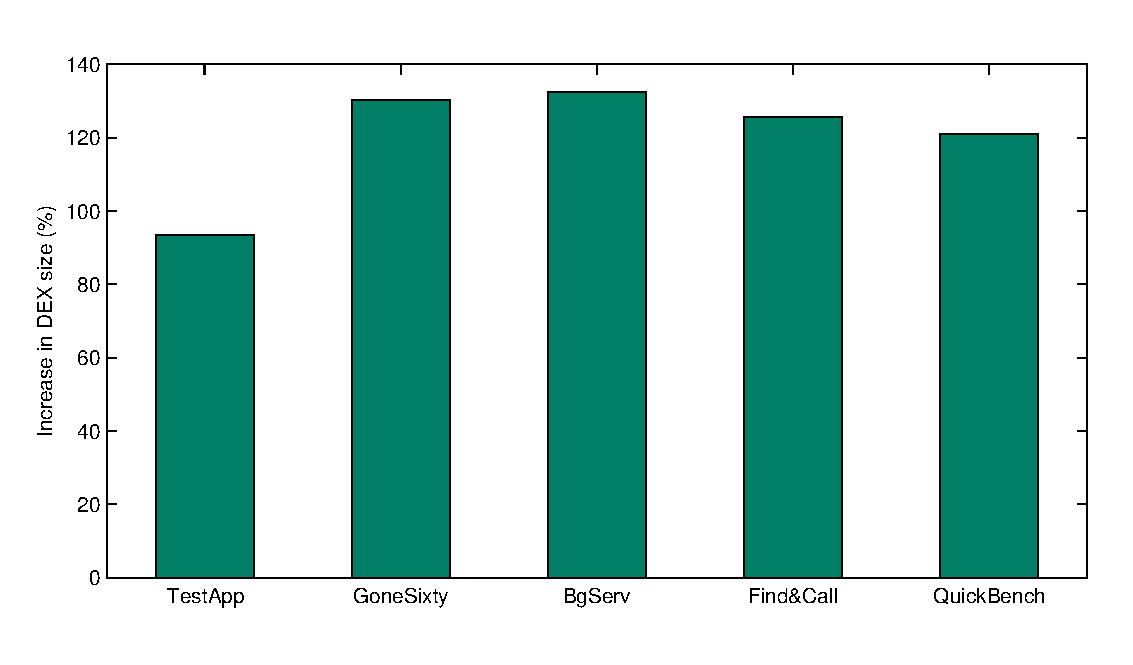
\includegraphics[width=0.7\textwidth]{figs/fig_eval_filesize.eps}
	}
	\caption{Increase in size of the executable DEX file caused by instrumentation.}
	\label{figure:Evalutaion_FileSize}
\end{figure}

Next we study the difference in the size of the instrumented file and the change in distribution of instruction types. Rather than being a performance metric, this creates a bigger picture of what flow analysis involves.

Figure~\ref{figure:Evalutaion_FileSize} shows that the overall size of the \emph{classes.dex} file approximately doubles, ranging between 90-140\% increase. This accounts for all sections of the file, i.e.\ bytecode, class definitions, constants, etc. On modern smartphones this should not be an issue as these executables are typically not bigger than few hundred kilobytes.

\begin{figure}
	\centerline{	
		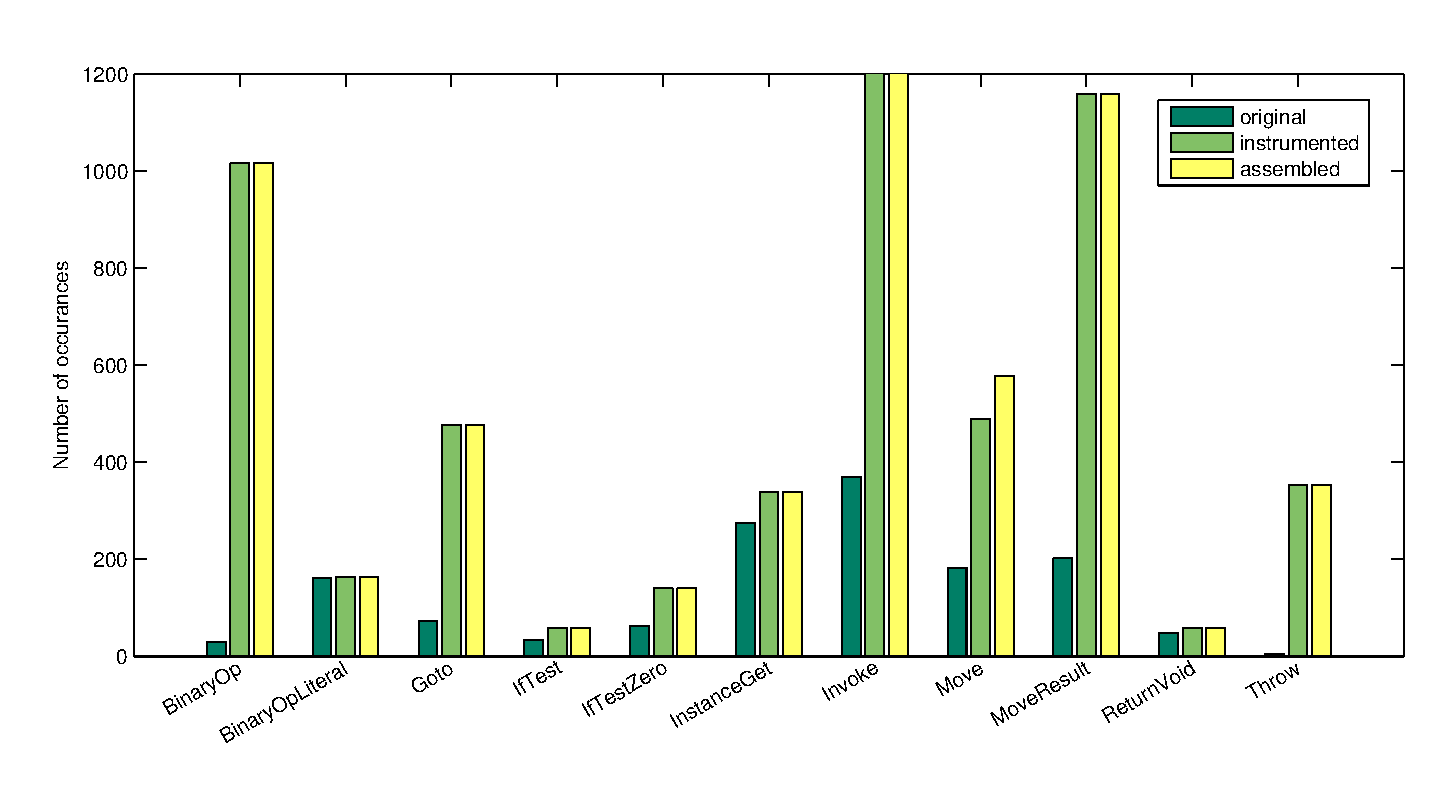
\includegraphics[width=\textwidth]{figs/fig_eval_codebloat.eps}
	}
	\caption{Number of occurrences of selected instructions in GoneSixty. First column represents the original count, second the state after application of instrumentation rules, and third the total count after assembling.}
	\label{figure:Evalutaion_CodeBloat}
\end{figure}

The change in distribution of opcodes is substantial. Figure~\ref{figure:Evalutaion_CodeBloat} shows some selected intermediate instruction types and how many times they appeared in the parsed, instrumented and post-assembly representation of the GoneSixty spyware. We see instructions that are virtually unaffected, like \verb$BinaryOpLiteral$ and \verb$ReturnVoid$ that are only added with the linked auxiliary classes, and that there are slightly more \emph{if} statements, mostly used for decisions during method calls and source/sink identification. On the other hand, the increase in the number of instructions directly involved in tainting is radical, especially \verb$invoke$ opcodes which jump from 400 to more than 3,h000 occurrences. These are nearly exclusively \verb$taint-get$ and \verb$taint-set$ calls, which go hand in hand with insertion of bitwise OR operations (\verb$BinaryOp$) to combine tags. Also notice that \verb$move$s are added during the assembly phase as a result of register spilling.

\section{Limitations}

The case studies above proved that taint tracking can indeed provide useful information about data leakage, but the approach naturally has its limits which will be discussed in this section. 

In terms of flow analysis, Dexter is by design restricted to tracking taint only from within a running VM and the code of the application. Hence it cannot compete with the system wide, VM modifying solution of TaintDroid that can propagate taint through the framework, between applications, through the filesystem, and also through reflective calls which Dexter simply treats as external. The same applies to dynamically loaded code, but since Dexter is implemented in Java, it could potentially be linked into the application and the code instrumented on-the-fly before being passed to the class loader.

As we saw in the BgServ case study, correct identification of sources and sinks requires information about \emph{all} framework methods that provide access to them. These definitions can be created very easily, but unfortunately this does not scale well. Covering all exotic ways of leaking data is therefore unrealistic in the light of the sheer size of the framework and its frequent updates. On the other hand, taint tracking systems are never perfectly leak-proof since there always exists a way of bypassing the taint propagation, for example through implicit data flow.

During testing, the greatest limiting factor of the actual implementation turned out to be the register allocating algorithm, which was incapable of dealing with very constrained methods. Even though SSA was implemented to solve this problem, conversion of IR to the internal representation of the standard JVM-DEX compiler, and making use of its existing advanced allocation and optimization techniques, would be a better solution but beyond the time frame of the project.

\section{Success Criteria}

\begin{description}
	\item \textbf{Criterion 1} \emph{Application must communicate with Android devices and be able to download/upload application packages (APKs).}

	The SDK's \verb$adb$ tool was used both to download and upload APKs and framework files. Shell commands were executed to list installed applications.

	\item \textbf{Criterion 2} \emph{Application must be able to extract content of APK files and to repackage them after instrumentation.}

	Packages are extracted, executables instrumented and new APKs generated and digitally signed.

	\item \textbf{Criterion 3} \emph{Specification of sources, sinks and sanitizers has to be designed and these properly identified by the instrumenting application.}

	Sources and sinks were defined by extending \verb$ExternalCallInstrumentor$ class. No sanitizers were needed in the end, but could easily be defined in the same way.

	\item \textbf{Criterion 4} \emph{Instrumentation of DEX files for both explicit and implicit flow analysis needs to be designed, implemented and shown to propagate taint correctly.}

	Instrumented applications perform full dynamic explicit flow analysis, support for implicit flows is limited to exception throwing due to spending more time than expected on the assembling process. Both were tested on tailored code snippets.

	\item \textbf{Criterion 5} \emph{Capabilities of the information-flow analysis must be demonstrated on examples of real applications.}

	Three applications known to spy on users were instrumented and shown to successfully identify data leakage. 
      
	\item \textbf{Criterion 6} \emph{Advantages and limitations of system-level integration versus per-application bytecode instrumentation for the purpose of taint-based flow analysis must be appraised.}

	Both approaches were thoroughly analyzed and their merits and limits explained.

	\item \textbf{Criterion 7} \emph{Performance must be compared to TaintDroid and overhead measured against the original code.}

	Overhead of individual operations was measured on the testing application. Benchmark downloaded from the application market was used for processor-bound performance measurements. Results were contrasted against those presented in the TaintDroid paper.
\end{description}

\cleardoublepage
\chapter{Conclusion}

\cleardoublepage

%%%%%%%%%%%%%%%%%%%%%%%%%%%%%%%%%%%%%%%%%%%%%%%%%%%%%%%%%%%%%%%%%%%%%
% the bibliography

\addcontentsline{toc}{chapter}{Bibliography}
\bibliography{refs}
\cleardoublepage

%%%%%%%%%%%%%%%%%%%%%%%%%%%%%%%%%%%%%%%%%%%%%%%%%%%%%%%%%%%%%%%%%%%%%
% the appendices
\appendix

\chapter{GoneSixty Security Report}
\label{chapter:Report_Gone60}
{\scriptsize\url{http://cms.avg-hrd.appspot.com/securitycenter/securitypost_20110927.html}}

\section{Overview}

\textbf{Name:} Gone in 60 Seconds \\
\textbf{Malware type:} Spyware \\
\textbf{Geo:} All around \\
\textbf{Score:} 3 \\
\textbf{Date Discovered:} 24.09.2011 \\
\textbf{Date Added:} 24.09.2011 \\

An Android application that can used as a spyware was found on Android Market

The application is Android cloud spyware that can be used by an attacker or not authorized user to take out personal info from the device such as contacts, messages, recent calls and history.

\section{Geeks Info}

\textbf{Method of Infection:} Installing an APK file \\
\textbf{Encrypted:} No \\
\textbf{Distribution Potential:} Low \\
\textbf{In the wild:} Yes \\
\textbf{Overall Risk Rating:} Low \\
\textbf{Damage Potential:} Low \\
\textbf{Reverse info:} Available \\
\textbf{Symptoms:} Taking personal information from target phone \\

\parbox{\textwidth}{
The developer of the app is 'CreativeDogs': \\
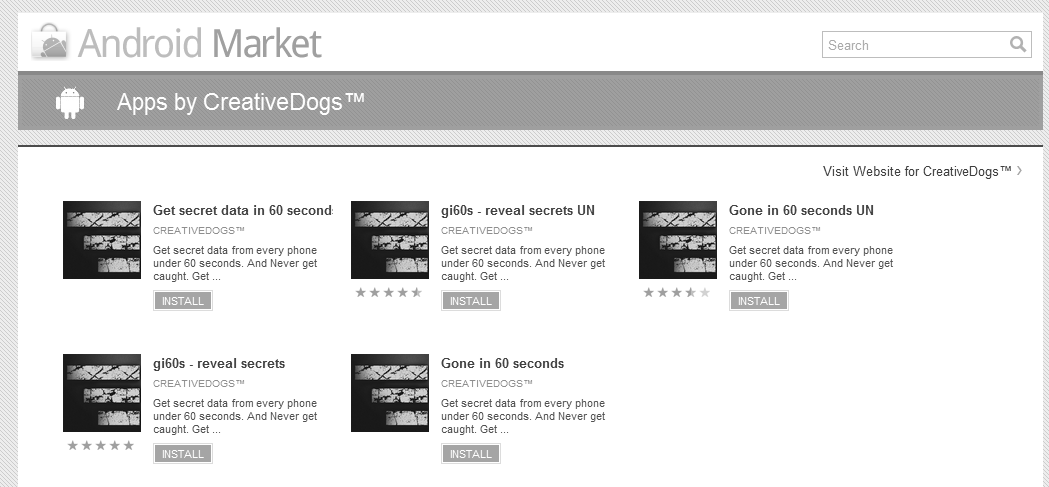
\includegraphics[width=0.95\textwidth]{figs/gone60_1.png}
}

\parbox{\textwidth}{
Details taken from the market: \\
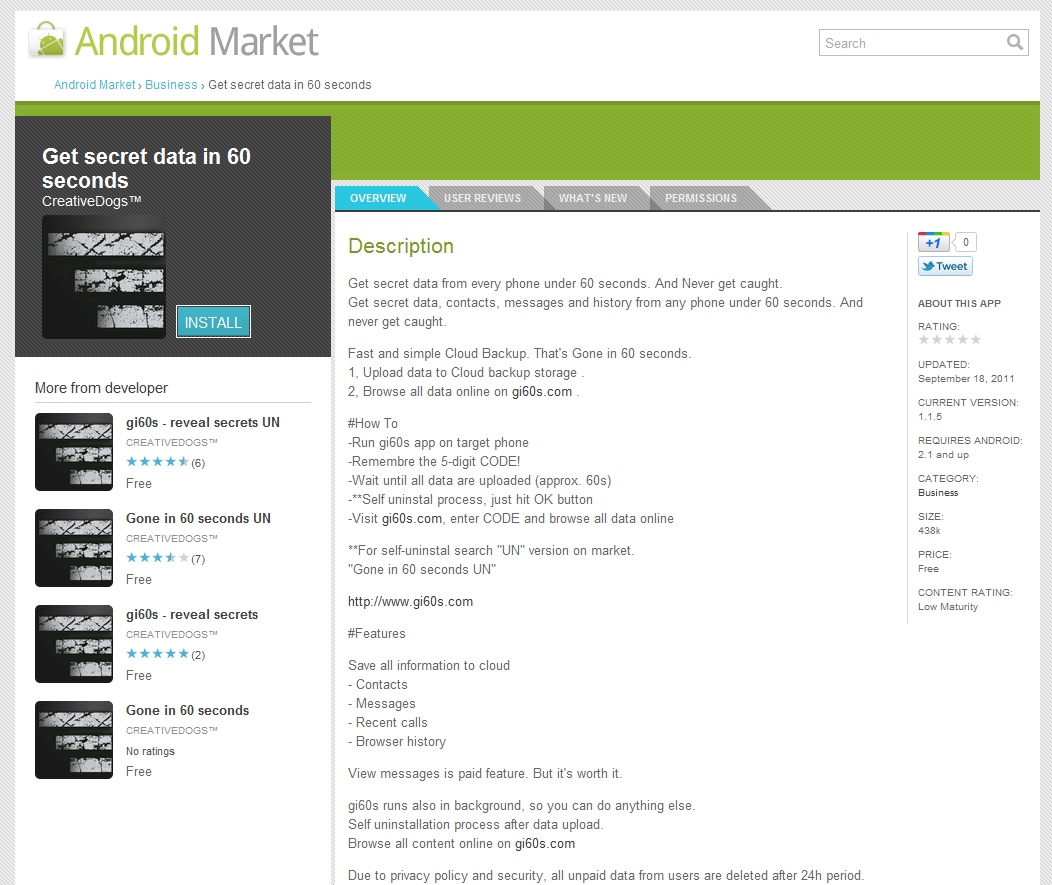
\includegraphics[width=0.95\textwidth]{figs/gone60_2.png}
}

\subsubsection{Package name}
\parbox{\textwidth}{
The package name of the application is 'com.gone603': \\
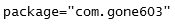
\includegraphics[width=0.3\textwidth]{figs/gone60_3.png} \\
\emph{Notice:} there are few variants of this app.
}

\subsubsection{Permissions}
\parbox{\textwidth}{
The spyware requests the permissions needed to what it intended to do: \\
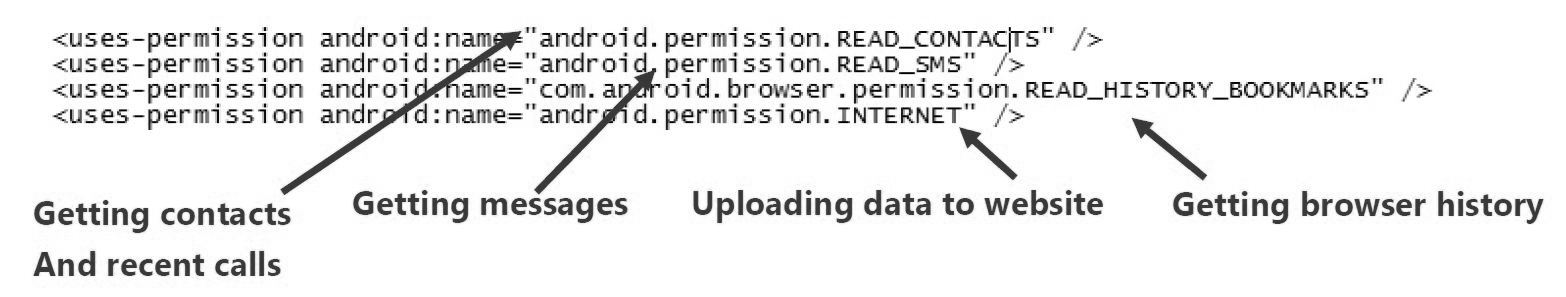
\includegraphics[width=\textwidth]{figs/gone60_4.JPG}
}

\subsubsection{Installing}
To activate the spyware the attacker needs to download and install it on the target phone.

\subsubsection{5 digit code}
\parbox{\textwidth}{
To activate the application the user needs to run it and remember the 5-digit code that will be later be used to browse the personal info taken in the spyware author. Below you can see how the application looks when running - the red area covers the code generated by the application: \\
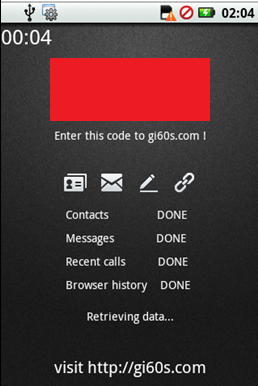
\includegraphics[width=0.5\textwidth]{figs/gone60_5.png}
}

\subsubsection{Running in the background}
The application runs in the background.

\subsubsection{Taking personal information from the target phone}
\parbox{\textwidth}{
The application gets its name from the time it takes for getting the data ad upload it to the spyware author's website. The flow and timing described below: \\
\texttt{Cloning contacts.. (10s)} \\
\texttt{Cloning messages.. (20s)} \\
\texttt{Cloning recent calls.. (10s)} \\
\texttt{Cloning browser history.. (15s)} \\
\texttt{Uploading data to gi60s.com.. (5s)} \\
}

\parbox{\textwidth}{
Here we can see the code part that is responsible for the flow: \\
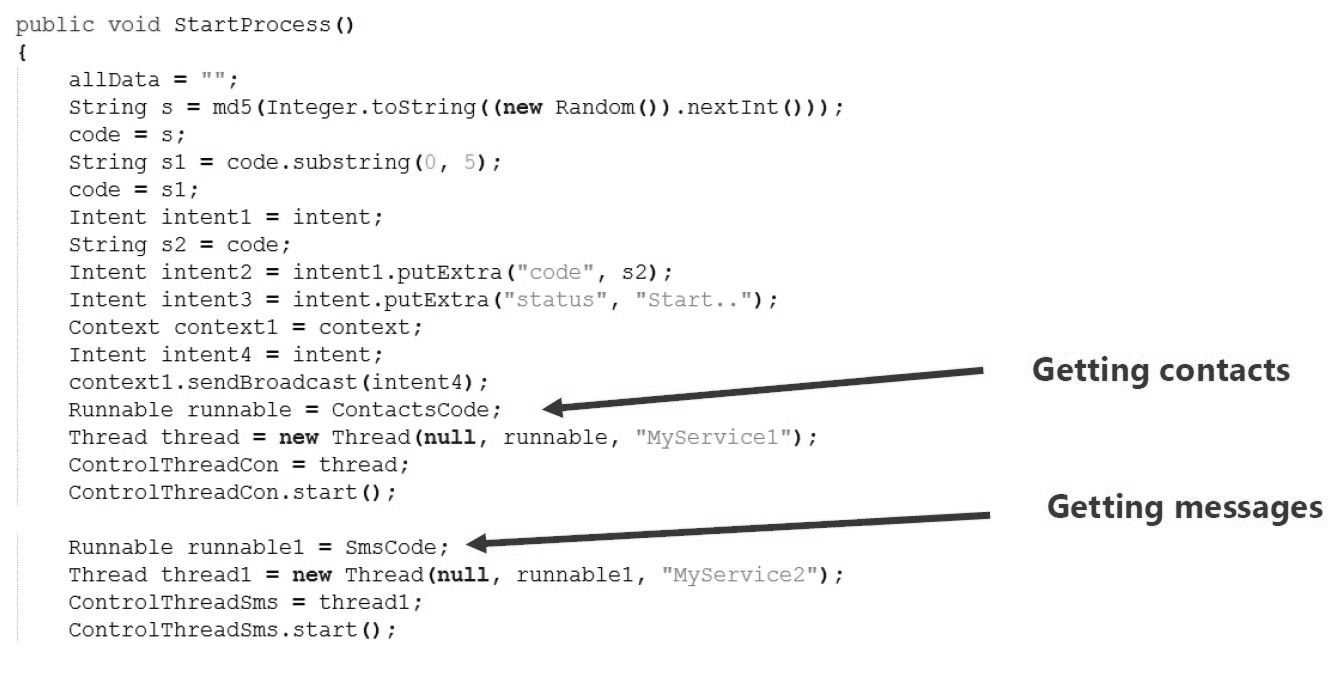
\includegraphics[width=\textwidth]{figs/gone60_6.JPG} \\
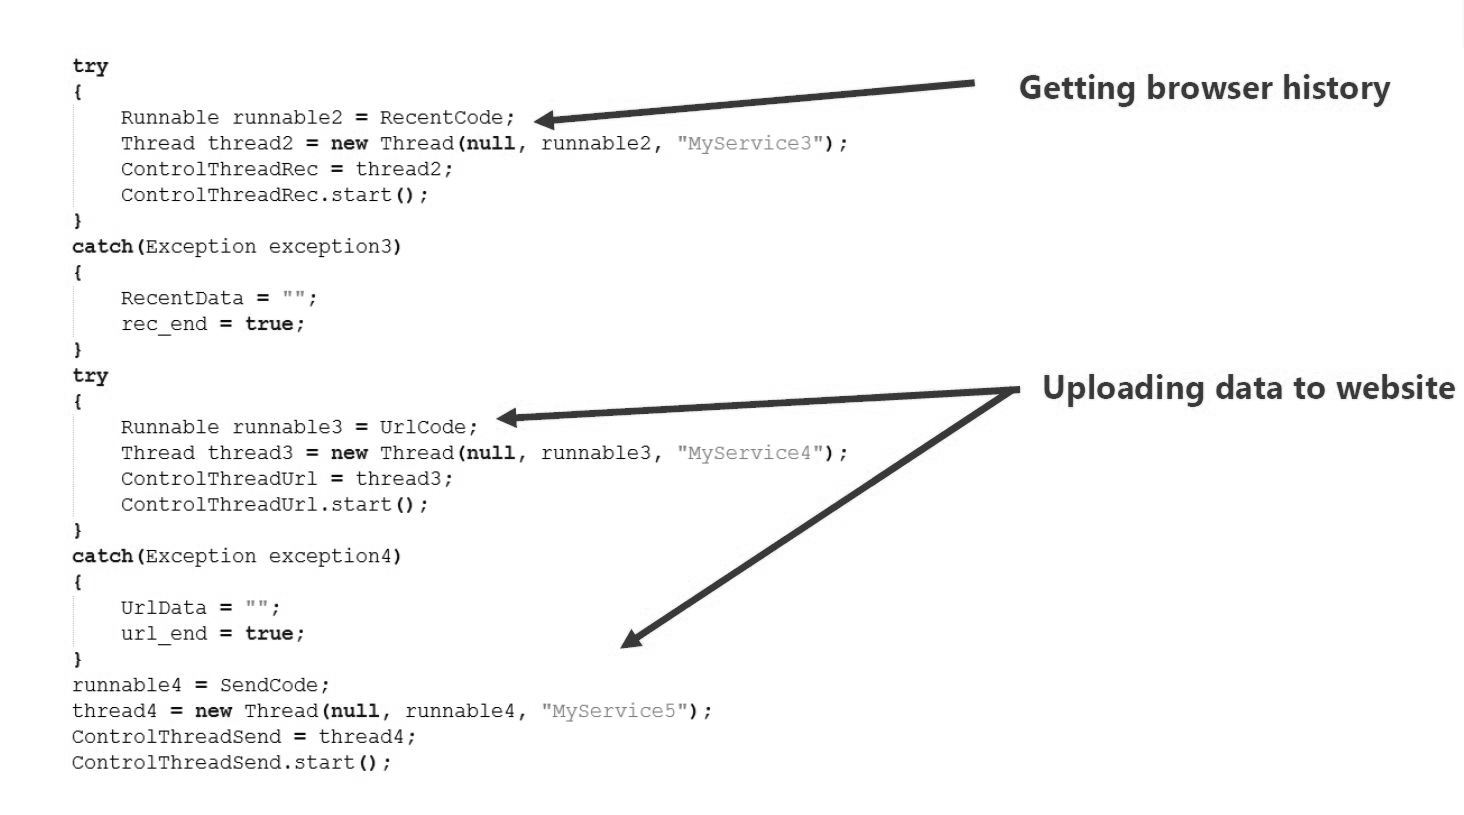
\includegraphics[width=\textwidth]{figs/gone60_6_2.JPG}
}

\parbox{\textwidth}{
Here we can see the code that takes the contacts (name + number) from the target phone: \\
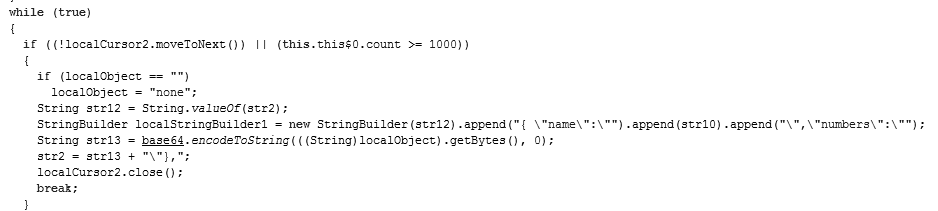
\includegraphics[width=\textwidth]{figs/gone60_7.png}
}

\parbox{\textwidth}{
Here we can see the code that takes the messages: \\
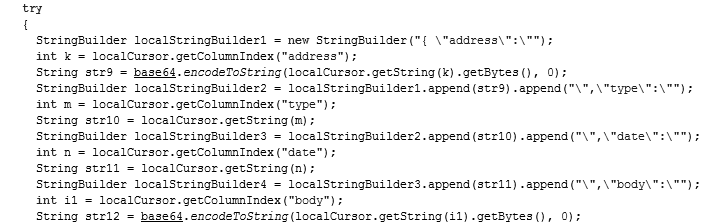
\includegraphics[width=\textwidth]{figs/gone60_8.png}
}

\parbox{\textwidth}{
Here we can see the code that takes the recent calls: \\
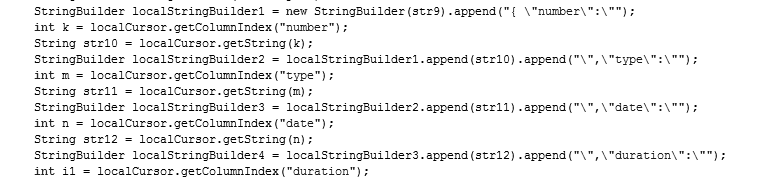
\includegraphics[width=\textwidth]{figs/gone60_9.png}
}

\parbox{\textwidth}{
Here we can see the code that takes the recent history: \\
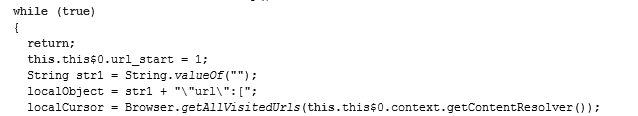
\includegraphics[width=\textwidth]{figs/gone60_10.png}
}

\subsubsection{Self-uninstallation}
\parbox{\textwidth}{
The developer declares that "The app automatically starts process of self-uninstallation". In reality, after running it the application still can be found on the device: \\
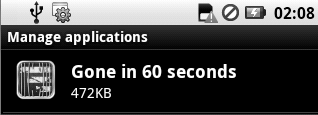
\includegraphics[width=0.5\textwidth]{figs/gone60_11.png}
}

\subsubsection{Getting the information taken from the target phone}
When you want to see the info taken from the device you need to browse to the application author website (giXXs.com), enter code and browse all contacts. To browse also messages, recent calls and history you need to pay the author 5\$.

\parbox{\textwidth}{
Here we can see the hard coded url of the author's website: \\
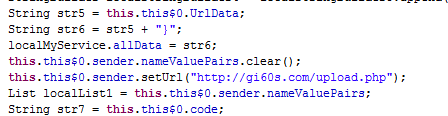
\includegraphics[width=0.8\textwidth]{figs/gone60_12.png}
}

\parbox{\textwidth}{
When you browse to the website there's a menu offer options: \\
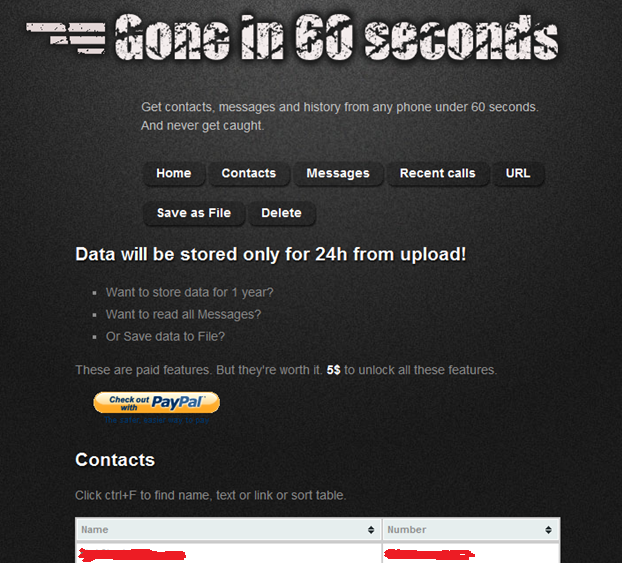
\includegraphics[width=0.75\textwidth]{figs/gone60_13.png}
}

\parbox{\textwidth}{
The authors of the application declare that the data will be stored only for 24h from upload. \\
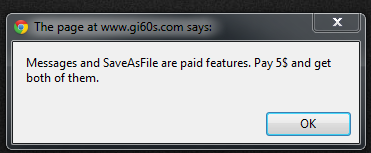
\includegraphics[width=0.5\textwidth]{figs/gone60_14.png}
}

\parbox{\textwidth}{
The following picture was taken from the author's website:\\
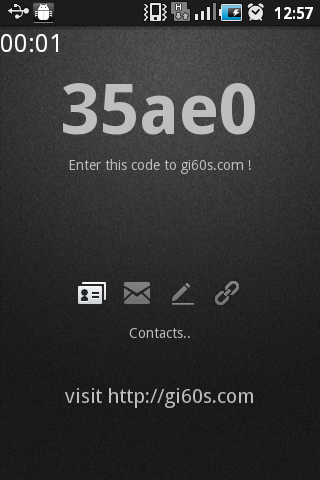
\includegraphics[width=0.5\textwidth]{figs/gone60_15.png}
}

\cleardoublepage

\chapter{BgServ Security Report}
\label{chapter:Report_BgServ}
\section{Summary}

\textbf{Discovered:} March 9, 2011 \\
\textbf{Updated:} March 10, 2011 5:41:31 AM \\
\textbf{Also Known As:} Troj/Bgserv-A [Sophos],	ANDROIDOS\_BGSERV.A [Trend] \\
\textbf{Type:} Trojan \\
\textbf{Infection Length:} 98,684 bytes \\
\textbf{Systems Affected:} Android

Android.Bgserv is a Trojan that opens a back door and transmits information from the device to a remote location. 

\textbf{\large Antivirus Protection Dates}
\begin{itemize}
	\item \textit{Initial Rapid Release version} March 9, 2011 revision 022
	\item \textit{Latest Rapid Release version} February 19, 2013 revision 016
	\item \textit{Initial Daily Certified version} pending
	\item \textit{Latest Daily Certified version} May 3, 2012 revision 004
	\item \textit{Initial Weekly Certified release date} March 9, 2011
\end{itemize}

\textbf{\large Threat Assessment} \\
\textbf{Wild}
\begin{itemize}
	\item \textit{Wild Level:} Low
	\item \textit{Number of Infections:} 0 - 49
	\item \textit{Number of Sites:} 0 - 2
	\item \textit{Geographical Distribution:} Low
	\item \textit{Threat Containment:} Easy
	\item \textit{Removal:} Easy
\end{itemize}
\textbf{Damage}
\begin{itemize}
	\item \textit{Damage Level:} Low
	\item \textit{Payload:} Opens a back door
\end{itemize}
\textbf{Distribution}
\begin{itemize}
	\item \textit{Distribution Level:} Low
\end{itemize}

\section{Technical Details}

The threat arrives bundled inside a legitimate application.

When the Trojan is executed, it collects the following information and saves it in the file [INSTALLATION PATH]/.hide/upload.xml:
\begin{itemize}
	\item IMEI
	\item Phone Number
	\item SMS Center
	\item Install Time
	\item System Version
\end{itemize}

It then uploads the collected information to the following remote site using the HTTP POST method: \\
{[}http://{]}www.youlubg.com:81/Coop/reques[REMOVED]

Next, it receives commands from the reply to the POST and saves the commands in the following file: \\
{[}INSTALLATION PATH{]}/.hide/serverInfo.xml

This allows the remote attacker to send SMS messages from the compromised device.

The threat also has the capability to block incoming SMS messages.

The threat may change the access port name (APN) to the following WAP network: \\
\textbf{Name:} cmwap \\
\textbf{APN:} cmwap \\
\textbf{Proxy:} 10.0.0.172 \\
\textbf{Port:} 80 \\
\textbf{MCC:} 460 \\
\textbf{MNC:} 02 \\
\textbf{Type:} default \\
\textbf{MMSC:} http://mmsc.monternet.com \\
\textbf{Number:} [EXISTING SIM OPERATOR NUMBER] \\

It then downloads a list of links from a remote site listed in the serverInfo.xml file and saves it as the following file: \\
{[}INSTALLATION PATH{]}/.hide/vedio.xml

It also downloads a file from a URL listed in the vedio.xml file and saves it as the following file: \\
{[}INSTALLATION PATH{]}/.hide/vedio\_file.3gp

It then restores the APN to its original settings.

The Trojan logs its activities in the following file for debugging purposes: \\
{[}INSTALLATION PATH{]}/.hide/log.txt

\textbf{Writeup By:} Mario Ballano and Kaoru Hayashi

\textbf{URL:} \url{https://www.symantec.com/security_response/writeup.jsp?docid=2011-031005-2918-99}
\cleardoublepage

\chapter{Project Proposal}


% Draft #1 (final?)

\vfil

\centerline{\Large Computer Science Project Proposal}
\vspace{0.4in}
\centerline{\Large How to write a dissertation in \LaTeX\ }
\vspace{0.4in}
\centerline{\large M. Richards, St John's College}
\vspace{0.3in}
\centerline{\large Originator: Dr M. Richards}
\vspace{0.3in}
\centerline{\large 14$^{th}$ October 2011}

\vfil


\noindent
{\bf Project Supervisor:} Dr M. Richards
\vspace{0.2in}

\noindent
{\bf Director of Studies:} Dr M. Richards
\vspace{0.2in}
\noindent
 
\noindent
{\bf Project Overseers:} Dr~F.~H.~King  \& Dr~A.~W.~Moore


% Main document

\section*{Introduction, The Problem To Be Addressed}


Many students write their CST dissertations in \LaTeX\ and
spend a fair amount of time learning just how to do that. The purpose of 
this project is to write a demonstration dissertation that explains in
detail how it done.  

This core proposal document will be augmented by a separately-printed
cover sheet at the front and a resource form at the end.  Additional
sheets for risk assessment and human resources may also need to be included.

This document will repeat much of the material that is summarised on the additional sheets.

\section*{Starting Point}

{\em Describe existing state of the art, previous work in this area, libraries and databases to be used.
Describe the state of any existing codebase that is to be built on.  }

I am already able to write prose using the English language. I have an online dictionary. etc..

\section*{Resources Required}

{\em A note of the resources required and confirmation of access.}

For this project I shall mainly use my own quad-core computer that runs Fedora Linux. Backup
will be to github and/or to an SVN repository on an external hard disk that is dumped to writable CD/DVD media.
I have another similar computer to hand should my main machine suddenly fail.
I require no other special resources.

\section*{Work to be done}

{\em Describe the technical work.}

The project breaks down into the following sub-projects:

\begin{enumerate}

\item The construction of a skeleton dissertation with the required 
structure. This involves writing the Makefile and makeing dummy files
for the title page, the proforma, chapters 1 to 5, the appendices and
the proposal.

\item Filling in the details required in the cover page and proforma.

\item Writing the contents of chapters 1 to 5, including examples
of common \LaTeX\ constructs.

\item Adding a example of how to use floating figures and encapsulated
postscript diagrams.

\end{enumerate}

\section*{Success Criterion for the Main Result}


The project will be a success if I have a completed dissertation with the correct chapter
titles and I have achieved my other success criterion, which is to blah ...



\section*{Possible Extensions}

{\em Potential further envisaged evaluation metrics or extensions.}

If I achieve my main result early I shall try the following alternative experiment or method of evaluation ...


\section*{Timetable: Workplan and Milestones to be achieved.}


{\em Perhaps list ten or so  two-week work-packages.}

Planned starting date is 16/10/2011.

\begin{enumerate}

\item {\bf Michaelmas weeks 2-4} Learn to use X. Read book Y. Read papers Z.

\item {\bf Michaelmas weeks 5-6} Do preliminary test of Q.

\item {\bf Michaelmas weeks 7-8} Start implementation of main task A.

\item {\bf Michaelmas vacation} Finish A and start main task B.

\item {\bf Lent weeks 0-2} Write progress report. Generate corpus of test examples. Finish task B.  

\item {\bf Lent weeks 3-5} Run main experiments and achieve working project.

\item {\bf Lent weeks 6-8} Second main deliverable here.

\item {\bf Easter vacation:} Extensions and writing dissertation main chapters.

\item {\bf Easter term 0-2:}  Further evaluation and complete dissertation.

\item {\bf Easter term 3:} Proof reading and then an early submission so as to concentrate on examination revision.

\end{enumerate}


 



\end{document}
